%!TEX root = ../thesis.tex
%*******************************************************************************
%****************************** Fifth Chapter *********************************
%*******************************************************************************

\chapter{Population-scale differentiation of iPSCs to a neuronal fate}
\label{chapter5}

The work described in \textbf{Chapter \ref{chapter4}} acted as a proof of principle study, where we demonstrated the feasibility of pooling cells from several lines prior to differentiating them towards an endodermal fate.
This means that in a single experiment we can obtain data from many independent donors, which in turn allows us to increase throughput of these studies thus enabling population-scale genetics to be performed.
Additionally, the single cell readouts make it possible to trace back the donor of origin of each cell, without the need for any barcoding.
We and others have shown that single cell RNA-seq can be used to map \gls{eqtl} and, despite the pooling, we retain enough cells per individual to do so successfully.
Finally, by profiling differentiations of several lines we can start to disentangle differences in differentiation efficiency across lines and experimental batches. \\

In this second study, we considered a larger-scale experiment in terms of both the number of donors (from 125 to 215) and cells (from around 40,000 to over 1 million) and apply similar principles to a more challenging differentiation protocol, considering iPSCs differentiating towards a midbrain neuronal fate.
First, the use of a droplet-based scRNA-seq technology allows us to assay a much larger number of cells, providing an overview of the cell types generated by this protocol. 
Second, the larger number of cell lines included, and the longer protocol, allows us to dive deeper into the differences across lines in terms of their efficiency to differentiate, and allows us to start exploring possible causes.
Lastly, the closer resemblance of the differentiated cells to primary tissues enables the exploration of the effects of disease-associated variants on relevant cell types both at a specific stage and across development. 

\newpage

\begin{Comment2}

\hspace{-3mm}\textbf{Contributions} This work is the result of a collaboration between the Stegle, Merkle, Marioni and Gaffney labs, and was funded by Open Targets (\url{https://www.opentargets.org}). 
The data was generated by Dan Gaffney’s lab at the Wellcome Trust Sanger Institute, and the experiments were led by Julie Jerber, who also contributed to the interpretation of the results. 
Madeline Lancaster generated and helped annotating the organoid data (section \ref{sec:organoids}). 
The statistical methods and analyses described in this chapter were co-supervised by Dan Gaffney and Oliver Stegle with some input from Florian Merkle, John Marioni and Natsuhiko Kumasaka. 
Daniel Seaton was originally the lead computational member of the team, and I replaced him more recently upon his departure from the lab.
As a result, Daniel Seaton processed the data and performed \gls{qc} (sections 5.2.2., 5.2.3). 
I then refined the cell type annotation and mapped our data to existing scRNA-seq datasets (section 5.2.4).
The work presented in sections 5.3 and 5.4 is intrinsically joint work between Daniel Seaton and myself, as these are originally analyses and observations made by Daniel which I later followed up and added to upon his departure from the lab, as well as in response to reviewers' comments.
Daniel Seaton and I developed and implemented the statistical methods to perform eQTL mapping (largely building on methods I had developed previously, described in Chapter 4) and I led the eQTL analysis, including comparison of different methods (section 5.5.1) and between results across cell types and other tissues (sections 5.5.2, 5.5.3). 
Finally, Natsuhiko Kumasaka ran the colocalisation analysis (section 5.6), the results of which Julie Jerber and I then explored and summarised.\\

The code for processing, analysing and plotting the data is open source and freely accessible here: \url{https://github.com/single-cell-genetics/singlecell\_neuroseq\_paper}.
Julie Jerber, Daniel Seaton, Dan Gaffney, Oliver Stegle and I wrote the manuscript, with input from Florian Merkle and John Marioni.
The paper \cite{jerber2020population} is available at : \url{https://www.nature.com/articles/s41588-021-00801-6} as:\\

Julie Jerber*, Daniel D. Seaton*, Anna S.E. Cuomo*, Natsuhiko Kumasaka, James Haldane, Juliette Steer, M Patel, D Pearce, M Andersson, Marc Jan Bonder, Ed Mountjoy, Maya Ghoussaini, Madeline A. Lancaster, the HipSci Consortium, John C. Marioni, Florian T. Merkle, Oliver Stegle, Daniel J. Gaffney. Population-scale single-cell RNA-seq profiling across dopaminergic neuron differentiation. \textit{Nature Genetics}, 2021 (* equal contributions). \\

I generated all figures presented in this chapter, except where indicated otherwise in figure legends. 

\end{Comment2}

\newpage

\section{Introduction}
\label{sec:neuroseq_intro}

As discussed in the previous chapters, genetic variation can significantly alter cell function, for example by leading to changes in gene expression. 
Human iPSCs are a promising cellular model for assessing the cellular consequences of human genetic variation across different lineages, developmental states and cell types. 
In particular, human iPSCs enable the study of developmental stages and stimulation conditions that would be challenging to access \textit{in vivo}. 
The creation of cell banks containing hundreds of iPSC lines \cite{kilpinen2017common} provides an exciting opportunity to carry out population-scale studies \textit{in vitro} \cite{cuomo2020single, strober2019dynamic, schwartzentruber2018molecular, alasoo2018shared}.
However, differentiating iPSCs is costly and labour-intensive, and differentiation experiments are difficult to compare due to substantial batch-to-batch variation (\textbf{section \ref{sec:ipsc}}).
Thus, experiments with more than a handful of cell lines remain a significant challenge.
Moreover, most iPSC differentiation protocols generate a heterogenous cell population, of which the target cell type represents only a subset \cite{d2019vitro, banovich2018impact, volpato2018reproducibility, nguyen2018single}. 
This variability in differentiation outcomes hampers efforts to assess the genetic contributions to cellular phenotypes.\\

Single cell profiling has enabled `multiplexed' experimental designs, where cells from multiple individuals are pooled together \cite{cuomo2020single, nguyen2018single}. 
Pooling improves throughput and allows experimental variability between differentiation batches to be rigorously controlled, by enabling cell type heterogeneity to be accounted for in downstream analysis. 
As we have seen in the previous chapter (\textbf{Chapter \ref{chapter4}}), multiplexed experimental designs have only been applied to one short differentiation protocol \cite{cuomo2020single}, which generated cells corresponding to very early stages of development, and thus have not captured differentiation progression toward a mature cell fate. 
Population-scale pooling during long-term differentiation offers the opportunity to examine the effect of common genetic variants on gene expression in each cell population produced over neural development, providing a foundation for future mechanistic studies.\\

Here, we develop and apply a multiplexing strategy to profile the differentiation and maturation of more than two hundred iPSC lines derived from the \gls{hipsci} towards a midbrain neural fate, including dopaminergic neurons (DA). 
DA are involved in motor function and other cognitive processes and play key roles in neurological disorders, including Parkinson’s Disease (PD)\footnote{Parkinson’s disease (PD) is a progressive neurodegenerative disorder, characterised by the loss of midbrain DA neurons. 
These neurons control motor behavior, and, as they degenerate, they result in several motor features of the disease, such as bradykinesia, rigidity, resting tremor, gait disturbances and postural instability \cite{lees2009parkinsons}.} \cite{osborn2017seq, stoddard2020stem}. 
Additionally, we expose some cells to an oxidative stress, which is thought to play a role in PD \cite{xiong2012mitochondrial}.

\newpage

\section{Single cell map of iPSCs neuronal differentiation}
\label{sec:neuroseq_overview}

\subsection{Experimental strategy and data generation}

215 feeder-free iPSC lines were selected from 215 unique, healthy, unrelated donors from the \gls{hipsci} consortium \cite{kilpinen2017common}.
Cells from multiple iPSC lines were pooled together in 17 pools, each containing cells from 7 to 24 lines.
24h after plating, neuronal differentiation of the pooled lines to a midbrain lineage was performed, as described by Kriks \textit{et al}. \cite{kriks2011dopamine}. 
To capture transcriptional changes during neurogenesis and neuronal maturation, \gls{scrnaseq} was performed from cells captured at day 11 (midbrain floorplate progenitors), day 30 (young post-mitotic midbrain neurons) and day 52 (more mature midbrain neurons). 
The three time points were selected based on the data available in the original paper, where molecular profiling, biochemical and electro-physiological data defined developmental progression of midbrain DA neurons \cite{kriks2011dopamine}. 
The timeline was aligned to theirs: in their paper they described days 11, 25, 50 as, respectively, midbrain DA progenitors, time of cell cycle exit, and long term neurons.
Day 30 was selected instead of day 25 to enrich for young post-mitotic neurons. 
Additionally, half of the cells on day 51 were exposed to a sub-lethal dose of rotenone, a chemical stressor that preferentially leads to DA death in models of PD \cite{xiong2012mitochondrial}.
Droplet-based \gls{scrnaseq} was performed using the 10X Genomics™ technology \cite{zheng2017massively}.
After \gls{qc}, a total of 1,027,401 cells was retained across 17 cell pools and four conditions - day 11, day 30, day 52 untreated and day 52 rotenone-treated (\textbf{Fig. \ref{fig:neuroseq_experimental_design}}).

\begin{figure}[h]

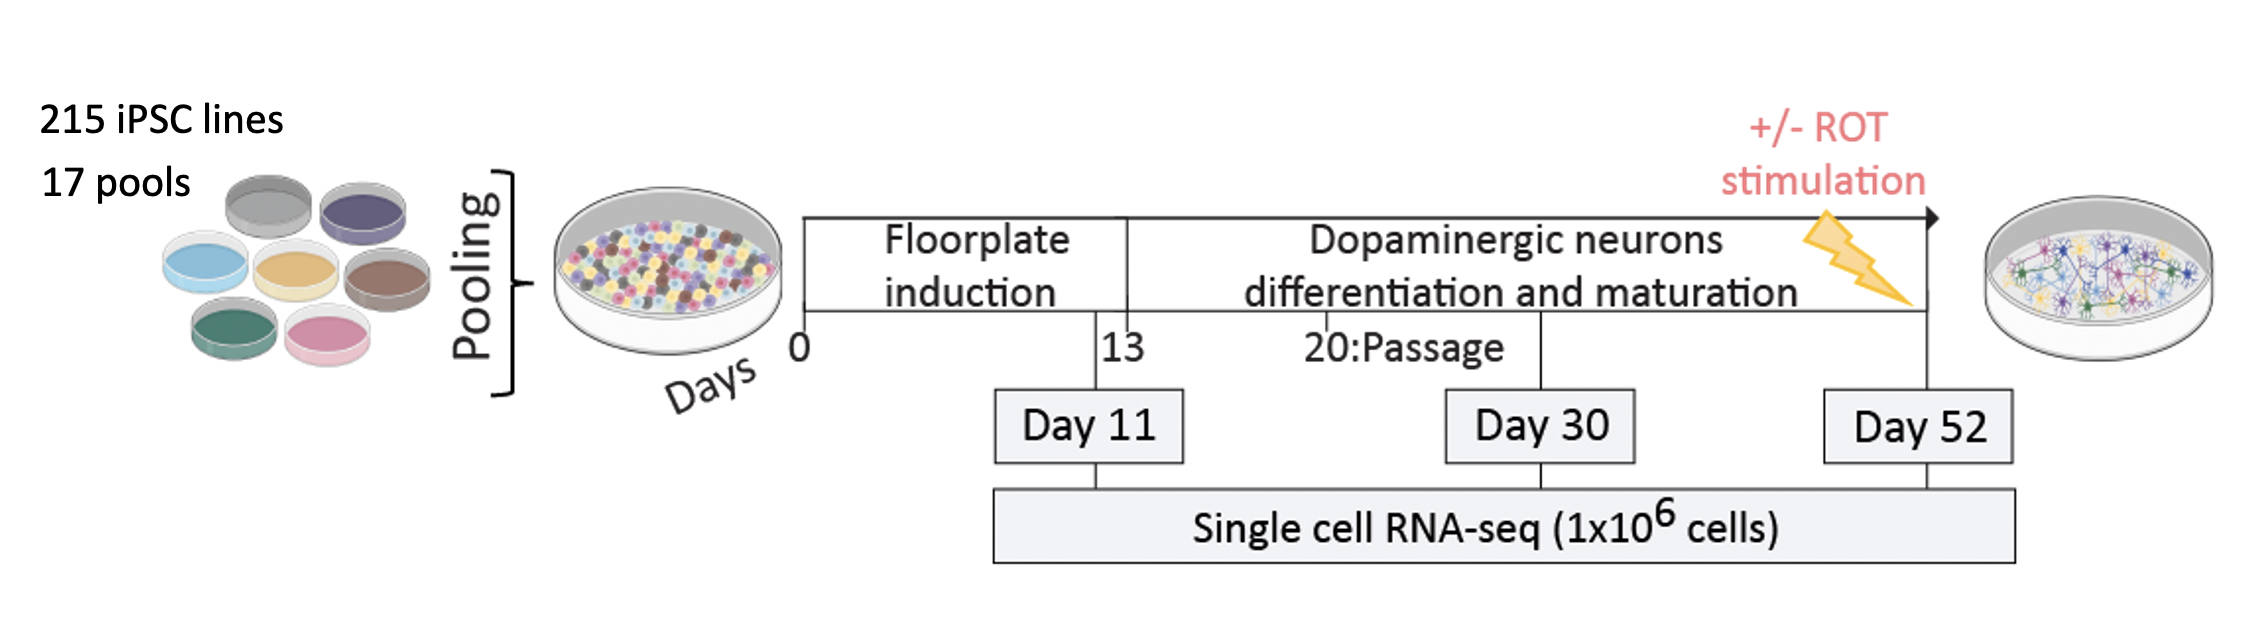
\includegraphics[width=16cm]{Chapter5/Fig/neuroseq_experimental_design.png}
\caption[Experimental Design]{\textbf{Experimental Design}.\\
Figure created by Julie Jerber.
Experimental design for pooled differentiations of iPSCs to midbrain dopaminergic neurons. 
The three time points (day 11, day 30, day 52) at which cells were collected for \gls{scrnaseq} profiling are shown. 
On day 51, 50\% of the cells were stimulated with rotenone (ROT) for 24h, to induce an oxidative stress.
Single cell RNA-seq data from 215 iPSC lines (for 215 donors) across 17 pools were collected for a total of over a million cells.}
\label{fig:neuroseq_experimental_design}
\end{figure}

\newpage

\subsection{Demultiplexing donors from pooled experiments}

For each of the 17 pooled experiments, donors (i.e. cell lines) were demultiplexed using demuxlet \cite{kang2018multiplexed}, considering genotypes of common exonic variants (MAF > 1\%) available from the HipSci bank, and a doublet prior of 0.05. 
Only single cells for which donor identification was successful were considered further. 
This QC step filtered out two kinds of droplet: droplets that contained two or more cells from different donors, and droplets containing no cells, but enough free-floating RNA to pass the CellRanger UMI filter.

\subsection{Normalisation, dimensionality reduction, and clustering}

Independent analysis of each time point allowed efficient batch effect correction, as all samples were from the same time point, containing similar mixtures of cell types.
Moreover, by reducing the number of cells analysed together, computational tasks were made more tractable.
In particular, the following steps were performed (at each time point): counts were normalised to the total number of counts per cell. 
Next, only genes with non-zero counts in at least 0.5\% of cells were retained and the top 3,000 highly variable genes were selected, after correcting for the mean-variance relationship in expression data. 
The first 50 principal components (PCs) were then calculated, and batch correction was applied on the level of PCs using Harmony \cite{korsunsky2019fast}, with each 10X sample treated as a distinct batch. 
UMAP and clustering was performed using the resulting transformed PCs. 
In particular, clustering was performed using Louvain clustering \cite{blondel2008fast} with 10 nearest neighbours. 
Data processing steps besides batch correction were performed using the Scanpy package \cite{wolf2018scanpy}. 
This identified a total of 26 clusters (6, 7 and 13 clusters at day 11, day 30, day 52, respectively \textbf{Fig. \ref{fig:neuroseq_clusters}}). \\

\begin{figure}[h]
\centering
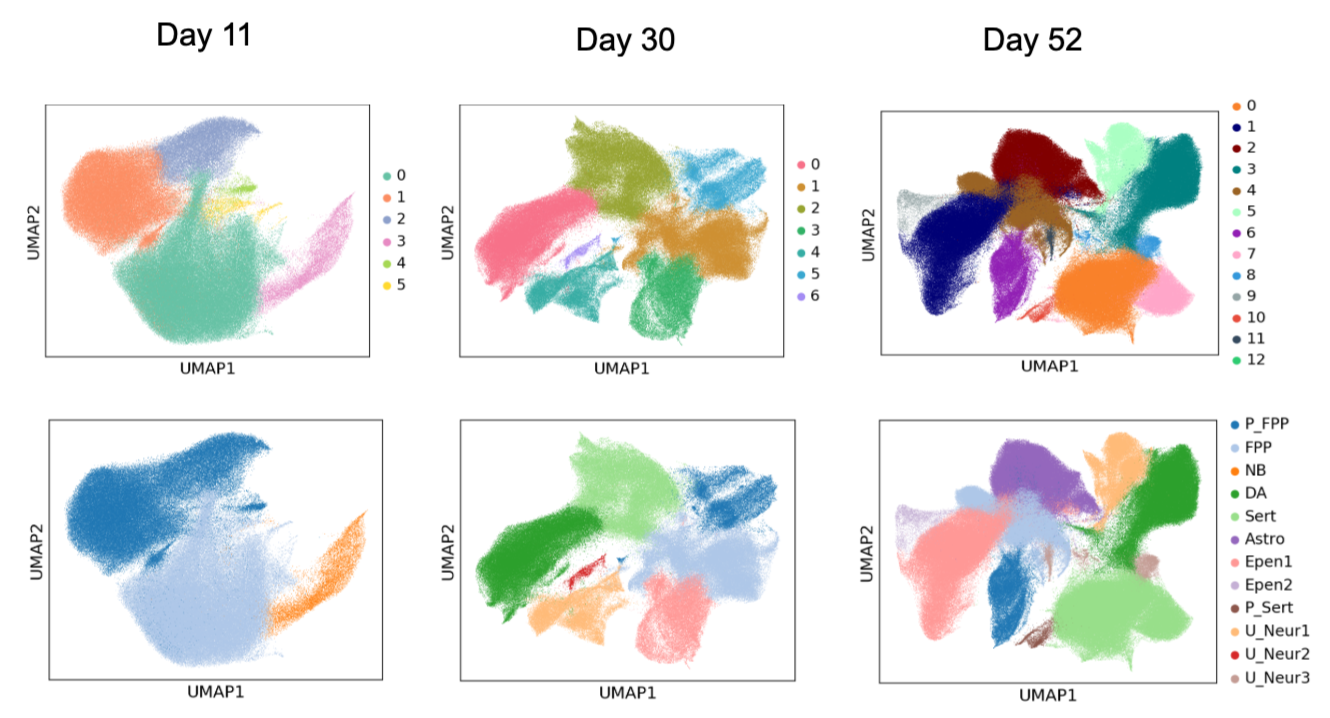
\includegraphics[width=16cm]{Chapter5/Fig/neuroseq_clusters_celltypes.png}
\caption[Clustering and cell type assignment]{\textbf{Clustering and cell type assignment}.\\
At each individual time point (day 11, day 30, day 52), cells were clustered using Louvain clustering \cite{blondel2008fast}, after normalisation and batch correction using Harmony \cite{korsunsky2019fast}.
Subsequently, clusters were annotated as cell types using known marker genes. 
When two clusters showed the same gene set enrichment they were computationally assigned to the same cell type identity. 
(a) UMAPs of cells sampled at each time point and coloured by cell clusters. 
(b) Same UMAPs as in (a), this time coloured by assigned cell types.
Astro: Astrocyte-like, DA: Midbrain dopaminergic neurons, Epen1,2: Ependymal-like, FPP: Floor plate progenitors, NB: Neuroblasts, P\_FPP: Proliferating floor plate progenitors, P\_Sert: Proliferating serotonergic-like neurons, Sert: Serotonergic-like neurons, U\_Neur1,2,3: Unknown neurons.}
\label{fig:neuroseq_clusters}
\end{figure}

Next, clusters were assigned to cell types using a set of literature-curated marker genes for major brain cell types (n=48 marker genes, see \textbf{Fig. \ref{fig:suppl_celltype_markers}}).
When two clusters showed the same gene set enrichment, they were assigned the same cell type identity (see next section).

\subsection{Cell type annotation}
Cell type annotation was carried out independently at each time point (day 11, day 30 and day 52).
For midbrain dopaminergic neurons, which is the target cell type of this protocol, I also performed additional analyses to verify the cell type identity.
In the next section, I describe the mapping from clusters (identified unbiasedly using the entire transcriptome) to cell types (using literature-curated gene markers).

\subsubsection{Day 11}

Three cell type populations were identified at day 11.
The two most prevalent ones, which constituted circa 96\% of all cells at this time point, were classified as proliferating and non-proliferating midbrain floorplate progenitors (both expressing \textit{LMX1A} and \textit{FOXA2} and expressing \textit{MIK67, TOP2A} when proliferating \cite{la2016molecular}, \textbf{Fig. \ref{fig:suppl_celltype_markers}}).
The third cell population (making up the remaining 4\% of day 11 cells) was labelled a neuroblast (NB) population, based on the expression of pro-neuronal genes \textit{NEUROD1}, \textit{NEUROG2} and \textit{NHLH1} \cite{bertrand2002proneural, lacomme2012neurog2}, \textbf{Fig. \ref{fig:neuroseq_clusters}, \ref{fig:suppl_celltype_markers}}).

\subsubsection{Day 30}

At day 30, cells with floorplate progenitor (23\%) and proliferating progenitor (7\%) identity could still be detected, whereas the neuroblast population was not seen any longer.

Additionally, five new cell types were identified.
Four of these additional cell types appeared neuronal and one was non-neuronal, as characterised by the expression (or lack thereof) of the pan-neuronal markers \textit{SNAP25} and \textit{SYT1} \cite{arenas2015make}.
Of the four neuronal populations, two could be assigned to a midbrain neuronal identity.
The first expressed canonical DA markers \textit{NR4A2}, \textit{PBX1}, and \textit{TMCC3} \cite{la2016molecular, park2006acquisition, ramonet2012park9} and was labelled as a population of midbrain dopaminergic neurons (DA, 27\%).
The second cell population expressed some serotonergic neuronal markers (\textit{TPH2, GATA2} \cite{cummings2019serotonergic}) and was categorised as serotonergic-like (Sert, 21\%) neurons. 
One additional large neuronal population (expressing \textit{SNAP25} and \textit{SYT1}), expressed both midbrain DA markers and cortical markers, and thus could not be assigned to a specific neuronal identity (Unknown neurons 1, around 8\%).
Finally, one smaller neuronal population (less than 2\%) could also not be assigned to a specific identity (Unknown neurons 2). 
The only non-neuronal cell type identified at day 30 expressed all the classical markers of ependymal cells (Ependymal 1 \cite{campbell2017molecular}, 11\%, \textbf{Fig. \ref{fig:neuroseq_clusters}, \ref{fig:suppl_celltype_markers}}). 

\subsubsection{Day 52}

At day 52, the cell types identified at day 30 were largely recapitulated (\textbf{Fig. \ref{fig:neuroseq_clusters}}).
Floorplate progenitors were present in smaller proportions (13 and 5\%).
In addition to DA, Sert, the mixed neuronal population 1 and the ependymal-like cell population 1, a population of astrocyte-like cells could be identified, which were unique to day 52 (Astrocyte-like \cite{sloan2017human, zhang2016purification}). 
Finally, three additional rare cell types (present in less than 2\% of cells sampled at any time point) were detected, namely a second ependymal-like population (Ependymal 2), a population of proliferating neuronal serotonergic-like cells (Prolif. serotonergic-like neurons), and one additional neuronal population which could not be annotated unambiguously (Unknown neurons 3, \textbf{Fig. \ref{fig:neuroseq_clusters}, \ref{fig:suppl_celltype_markers}}). \\

We note that in general, we are careful to clarify that these are \textit{in vitro}-generated cell types, which will not be exactly the same as their \textit{in vivo} counterpart, especially for cell types that were not the target of the protocol used - thus the nomenclature xx-like, e.g. astrocyte-like, and serotonergic-like.
In the next section I discuss this further for the two cell populations which we assigned to a midbrain neuronal identity.

\subsubsection{Serotonergic-like neuronal population}

First, the population we call serotonergic-like was an especially hard one to define.
Serotonergic neurons are located in the same brain region as dopaminergic neurons 
(the midbrain), and share some common functions and gene markers.
However, whilst dopaminergic neurons have been very well characterised, partly because of their involvement in PD, serotonergic neurons have not been studied as much, and there are no well defined markers (at least not in human, whereas there are a few mouse studies \cite{cummings2019serotonergic}).
Additionally, there is no \textit{in vivo} single cell reference dataset.
The only study containing a human serotonergic neuronal cell population to the best of my knowledge is La Manno \textit{et al}. \cite{la2016molecular}, which contained only 14 cells.
In the same study they also derive midbrain neurons from human iPSCs, but do not obtain any serotonergic neurons.
Since our population expressed some, but not all, canonical serotonergic markers, we could not unambiguously say that these were serotonergic neurons, hence the name serotonergic-like.

\subsubsection{Dopaminergic neuronal population}

In contrast, human midbrain dopaminergic neurons are much better annotated, and in particular there exist published \textit{in vivo} datasets we can compare to.

Specifically, to confirm the dopaminergic identity of our DA cell population, I compared our cells to three datasets: human iPSC-derived dopaminergic neurons and human fetal cells from La Manno \textit{et al.} \cite{la2016molecular} and substantia nigra samples from post-mortem donors from Welch \textit{et al}. \cite{welch2019single}. \\

To perform the mapping, I performed joint PCA (using the multiBatchPCA from the batchelor package, implemented in R) and batch correction (using MNN \cite{haghverdi2018batch}) of log-normalised counts (using scater \cite{mccarthy2017scater}) from our data and each of the three reference datasets. 
The set of genes used was the union of 2,000 highly variable genes (HVGs, using the trendVar function from scran) from our data and 2,000 HVGs from the reference dataset. 
Next, I asked which reference cell each of our cells was most similar to (i.e. ‘mapped to', using queryKNN as implemented in BiocNeighbors, with k=1 nearest neighbour).\\

I mapped our DA cells to the set of all neurons from each of three datasets.
First, I compared to the La Manno \textit{et al}. iPSC data, and found that 99\% of our DA cells mapped to the `iDAb' population.
Second, to the La Manno \textit{et al}. embryonic data. 
85\% of our DA cells mapped to one of the dopaminergic populations in the reference, i.e. 39\% to `hDA1', 36\% to `hDA2', and 10\% to `hDA0'.
Finally, we mapped our DA cells to the Welch \textit{et al} post-mortem data, and found that for 91\% cells mapped to `NEUROdop', with the remaining 8\% mapping to a population of inhibitory neurons, `NEUROinh1'.
These combined analyses provide confidence in the identity of DA neurons from our iPSC differentiation model.

\newpage

\subsection{Data overview}

For visualisation purposes, we also performed a combined analysis of a random subsample of 20\% of all cells (after QC) from the three time points.
In this case, the Harmony batch correction was performed across pools (rather than across individual 10X samples, as before).
A joint UMAP projection of cells collected across all time points, stimuli and lines revealed broad co-clustering of cell types (using the labels described previously, see \textbf{Fig \ref{fig:neuroseq_clusters}}), but with noticeable differences between time points and stimuli (\textbf{Fig. \ref{fig:neuroseq_overview}}). \\

Substantial variation in the cell type proportions could be observed, across time points and stimuli (\textbf{Fig. \ref{fig:neuroseq_overview}}). 
For example, the proportion of DA cells was significantly reduced upon rotenone stimulation (30\% reduction, Fisher’s exact test, p value = $2.2 \times 10^{-16}$), which was consistent with previous observations that dopaminergic neurons are most affected by apoptosis due to oxidative stress \cite{sherer2003mechanism, knonagel1992autologous, cannon2009highly}.
Collectively, our population-scale \gls{scrnaseq} analysis revealed a diverse repertoire of cell types, enabling both the study of cell line differentiation propensity (\textbf{sections \ref{sec:neuroseq_diff_eff}, \ref{sec:neuroseq_ips}}) and the identification of genetic variants that affect expression in a cell type-specific manner (\textbf{sections \ref{sec:neuroseq_eqt}, \ref{sec:neuroseq_coloc}}). 
\\ 

\begin{figure}[h]
\centering
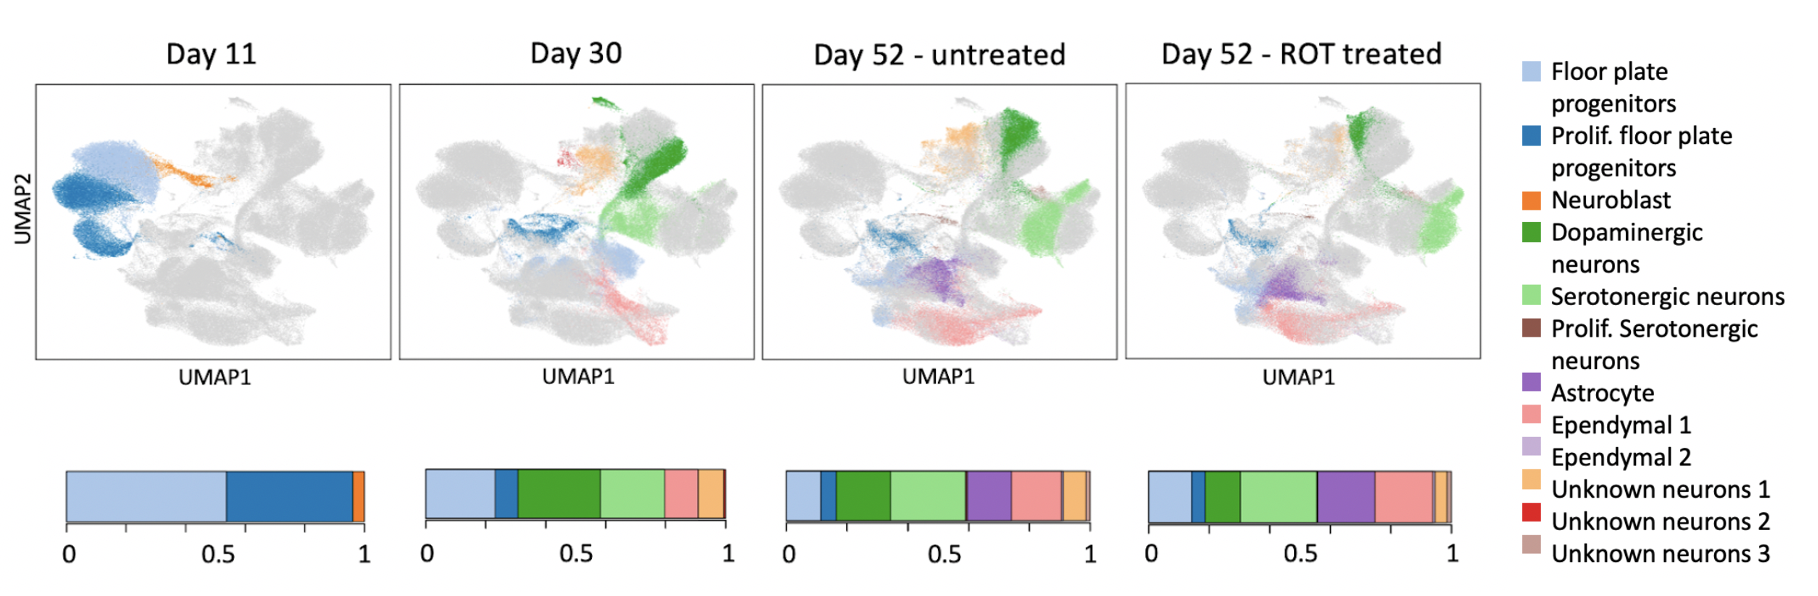
\includegraphics[width=17cm]{Chapter5/Fig/neuroseq_overview.png}
\caption[Overview of study]{\textbf{Overview of study}.\\
Top: UMAP plots of a subset of 205,416 cells assayed (20\% of the total), coloured by cell type identity. 
Cells that were not collected at a given (time point, stimulus) condition are shown in light grey. 
ROT: rotenone; Prolif: Proliferating. 
Bottom: Bar plots showing, for each condition, the fraction of cells assigned to each cell type.}
\label{fig:neuroseq_overview}
\end{figure}

\newpage

\section{Line-to-line variation in neural differentiation efficiency}
\label{sec:neuroseq_diff_eff}

The great diversity of cell types generated by this protocol raised the question of whether it may be driven by variation in differentiation outcome between different iPSC lines, which, as we have seen, is prevalent in iPSC differentiation studies (see \textbf{section \ref{sec:endodiff_differentiation_efficiency}} as well as other studies e.g. \cite{d2019association, volpato2018reproducibility}). 
Yet, as we discussed, the biological basis for this high variability in differentiation outcomes between lines remains largely obscure, which complicates efforts to rationally select cell lines for different applications. 
Here, we found substantial variation in the proportions of different cell types produced by different iPSC cell lines at each time point. 
For example, the proportion of day 52 untreated cells assigned to DA neurons ranged from 1\% to 100\% from line to line.
(\textbf{Fig. \ref{fig:neuroseq_line_variation}}).

\begin{figure}[h]
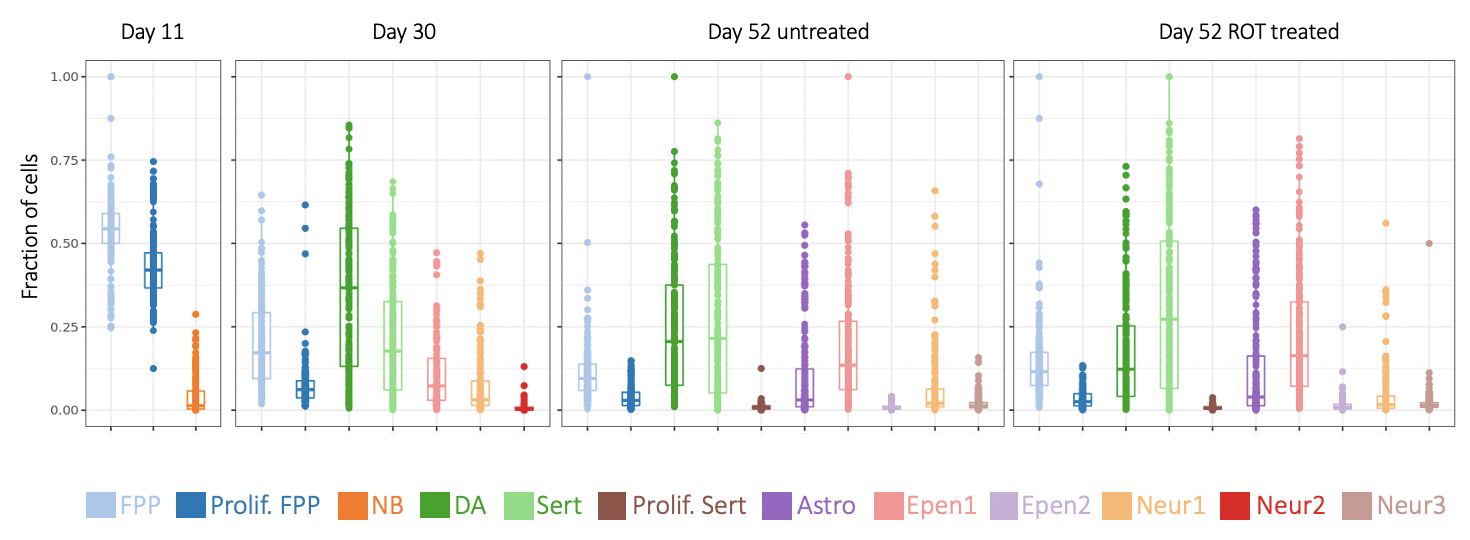
\includegraphics[width=15.5cm]{Chapter5/Fig/neuroseq_line_celltype.png}
\caption[Cell type fractions across lines]{\textbf{Cell type fractions across lines}.
Box plots showing, for each cell type, the proportions of that cell type across cell lines at day 11, day 30, untreated day 52, rotenone (ROT) treated day 52. 
Each point indicates a different cell line. 
Astro: Astrocyte-like, DA: Dopaminergic neurons, Epen1,Epen2: Ependymal-like, FPP: Floor Plate Progenitors, NB: Neuroblasts, P\_FPP: Proliferating FPP, Sert: Serotonergic-like neurons, P\_Sert: Proliferating Sert, U\_Neur: Unknown Neurons.}
\label{fig:neuroseq_line_variation}
\end{figure}


Looking at the cell type fractions per cell line and pool across time points, we observed a bimodality in the data, with roughly 2/3 of the iPSC lines mostly making DA and Sert at day 30 and day 52, and the other 1/3 making very few midbrain neurons but many glial cells (Ependymal-like and Astrocyte-like) instead (\textbf{Fig. \ref{fig:neuroseq_diff_efficiency}}).
When we performed \gls{pca} of such cell type fractions matrix, we identified the proportion of midbrain neurons (DA and Sert) on day 52 as the largest axis of variation (PC1, 47\% variance, \textbf{Fig. \ref{fig:neuroseq_diff_efficiency}}). 
Since DA and Sert cells are derived from similar progenitor populations \textit{in vivo}, it is not surprising that both populations are observed in our differentiation experiment \cite{ye1998fgf, cao2017characterization}. 
This motivated us to estimate a `neuronal differentiation efficiency' for each iPSC line, defined as the sum of the fractions of DA and Sert cells produced on day 52 (\textbf{Fig. \ref{fig:neuroseq_diff_efficiency}}). 

\begin{figure}[htbp]
\centering
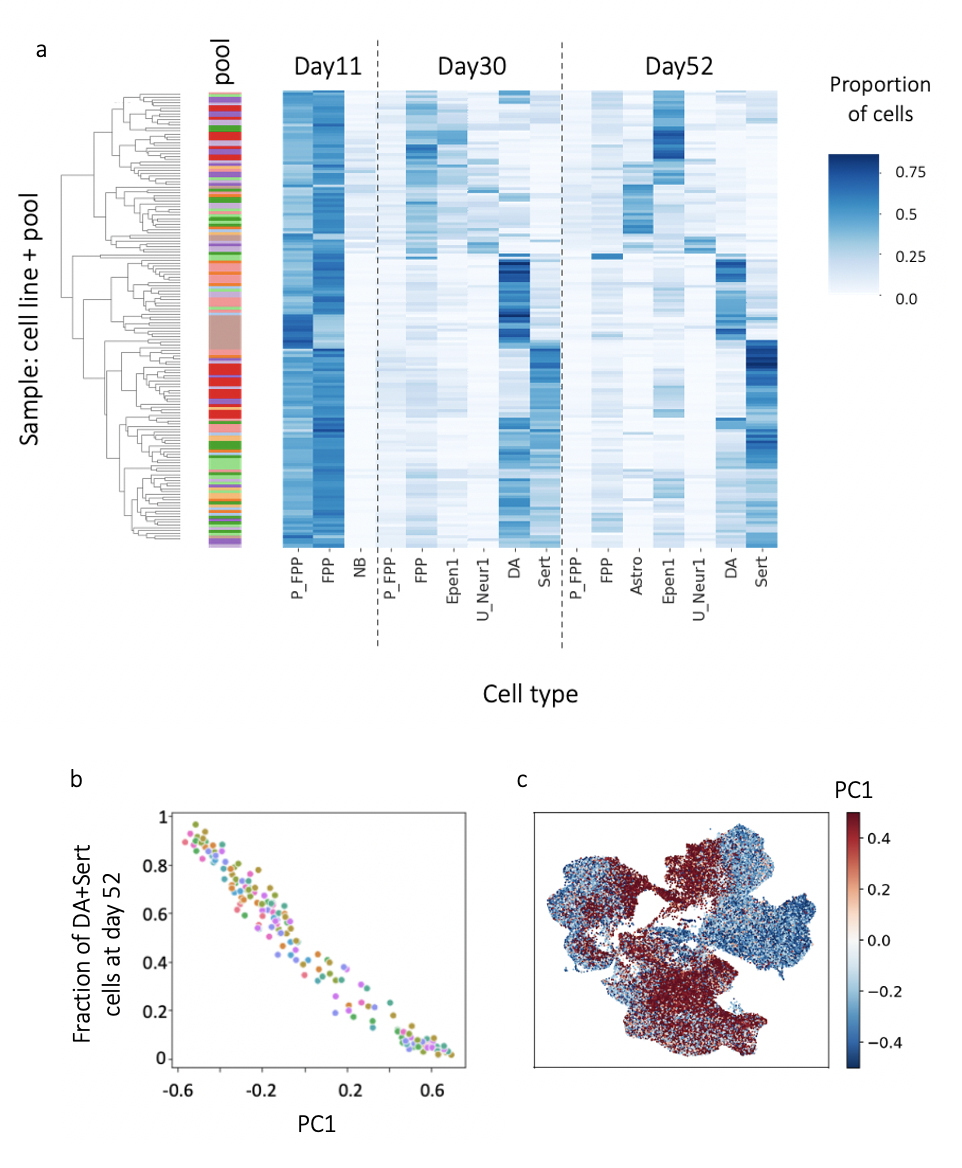
\includegraphics[width=14cm]{Chapter5/Fig/neuroseq_define_diff_efficiency.png}
\caption[Definition of neuronal differentiation efficiency]{\textbf{Distribution of cell proportions at day 52 and definition of neuronal differentiation efficiency}.
Cell proportions were generated for each cell type and time point for all combinations of cell lines and pools with at least 10 cells at all time points (10 pools). 
(a) Heatmap of the resulting cell proportion matrix. 
Pools are shown in the first bar and the colours indicate in which of the 10 pools each line was differentiated. 
Rows (i.e. cell line, pool combinations) were hierarchically clustered according to Euclidean distance. 
(b) Comparison of the first principal component (PC1) to the sum of fractions of dopaminergic and serotonergic-like neurons present on day 52.
(c) UMAP of cells included in (a), coloured by PC1.
Astro: Astrocyte-like, DA: Dopaminergic neurons, Epen1: Ependymal-like, FPP: Floor Plate Progenitors, NB: Neuroblasts, P\_FPP: Proliferating FPP, Sert: Serotonergic-like neurons, U\_Neur: Unknown Neurons.}
\label{fig:neuroseq_diff_efficiency}
\end{figure}

\clearpage

We assessed the reproducibility of this measure of neuronal differentiation efficiency using data from 32 lines that were differentiated twice, in two different pools. 
Importantly, we found that iPSC line neuronal differentiation efficiency defined in this way was highly reproducible between different pools (Pearson's R = 0.75; p value = $2 \times 10^{-6}$, \textbf{Fig. \ref{fig:neuroseq_diff_eff_replication}}).

\begin{figure}[h]
\centering
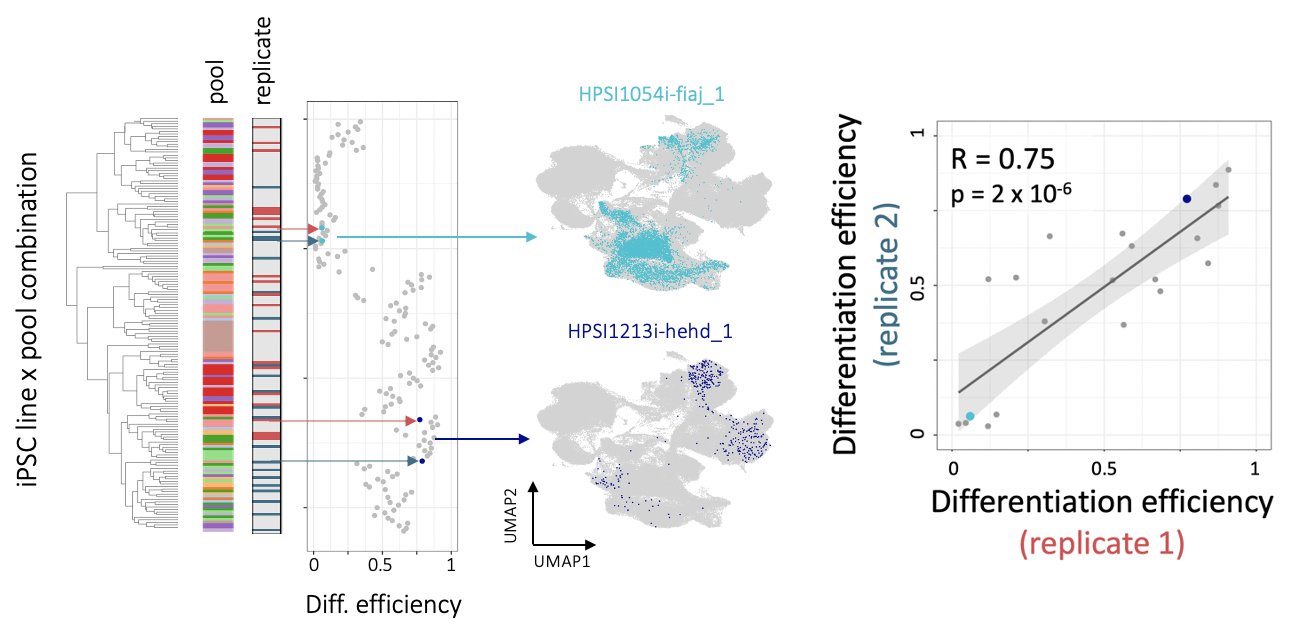
\includegraphics[width=15.5cm]{Chapter5/Fig/neuroseq_diff_eff_replication.png}
\caption[Reproducible neuronal differentiation efficiency]{\textbf{Reproducible variation in differentiation trajectories}.\\
(left) Hierarchical clustering of (cell line, pool) combinations (same as \textbf{Fig. \ref{fig:neuroseq_diff_efficiency}}) by neuronal differentiation efficiency. 
Colours in the first bar indicate in which of 10 pools (for which we had data at all time points, used to define neuronal differentiation efficiency) each line was differentiated. 
Differentiation replicates for lines present in two pools, are indicated in the second bar (red for replicate 1 blue for replicate 2).
(middle) UMAPs, highlighting the distributions of cells on day 52 for two selected cell lines with low and high differentiation efficiencies respectively (HPSI0514i-fiaj\_1, in seagreen and HPSI1213i-hehd\_1, in dark blue).
(right) Scatter plot showing estimated neuronal differentiation efficiency between differentiation replicates (i.e. cell lines differentiated in two different pools, out of the 10 pools considered here, n=21). 
Highlighted are the same two cell lines.}
\label{fig:neuroseq_diff_eff_replication}
\end{figure}

\subsection{Organoids}
\label{sec:organoids}

Given the robustness of our measure of neuronal differentiation efficiency, we next wondered if it was generalisable to other differentiation approaches. 
We therefore differentiated a pool of 18 lines (pool 4) into cerebral organoids for 113 days (as previously described in Lancaster \textit{et al}. \cite{lancaster2017guided}) and profiled the resulting cell populations using \gls{scrnaseq} (11,445 cells). 
The same steps of dimensionality reduction, batch correction and clustering applied to the midbrain dataset were applied to the cerebral organoid data. 
These steps identified eight clusters that were labelled as different cell types (i.e. neuronal cells, intermediate progenitor cells, radial glial progenitor cells, satellite cells, mesenchymal cells, myotube and Wnt and PAX7 positive cells) using 24 marker genes (\textbf{Fig. \ref{fig:neuroseq_organoids}}).
We found that the proportion of brain cell types (all neuronal, glial, and neural progenitor cells) produced by each line in the cerebral organoids was strongly correlated with neuronal differentiation efficiency as estimated from the dopaminergic differentiation (R = 0.94; p value = $2 \times 10^{-5}$; n=12). 
Taken together, these results strongly suggest that variation in iPSC neuronal differentiation efficiencies arise primarily due to cell-intrinsic factors. 
Furthermore, the consistency of neuronal differentiation efficiency suggests that these properties extend to neuronal differentiation more generally.

\begin{figure}[htbp]
\centering
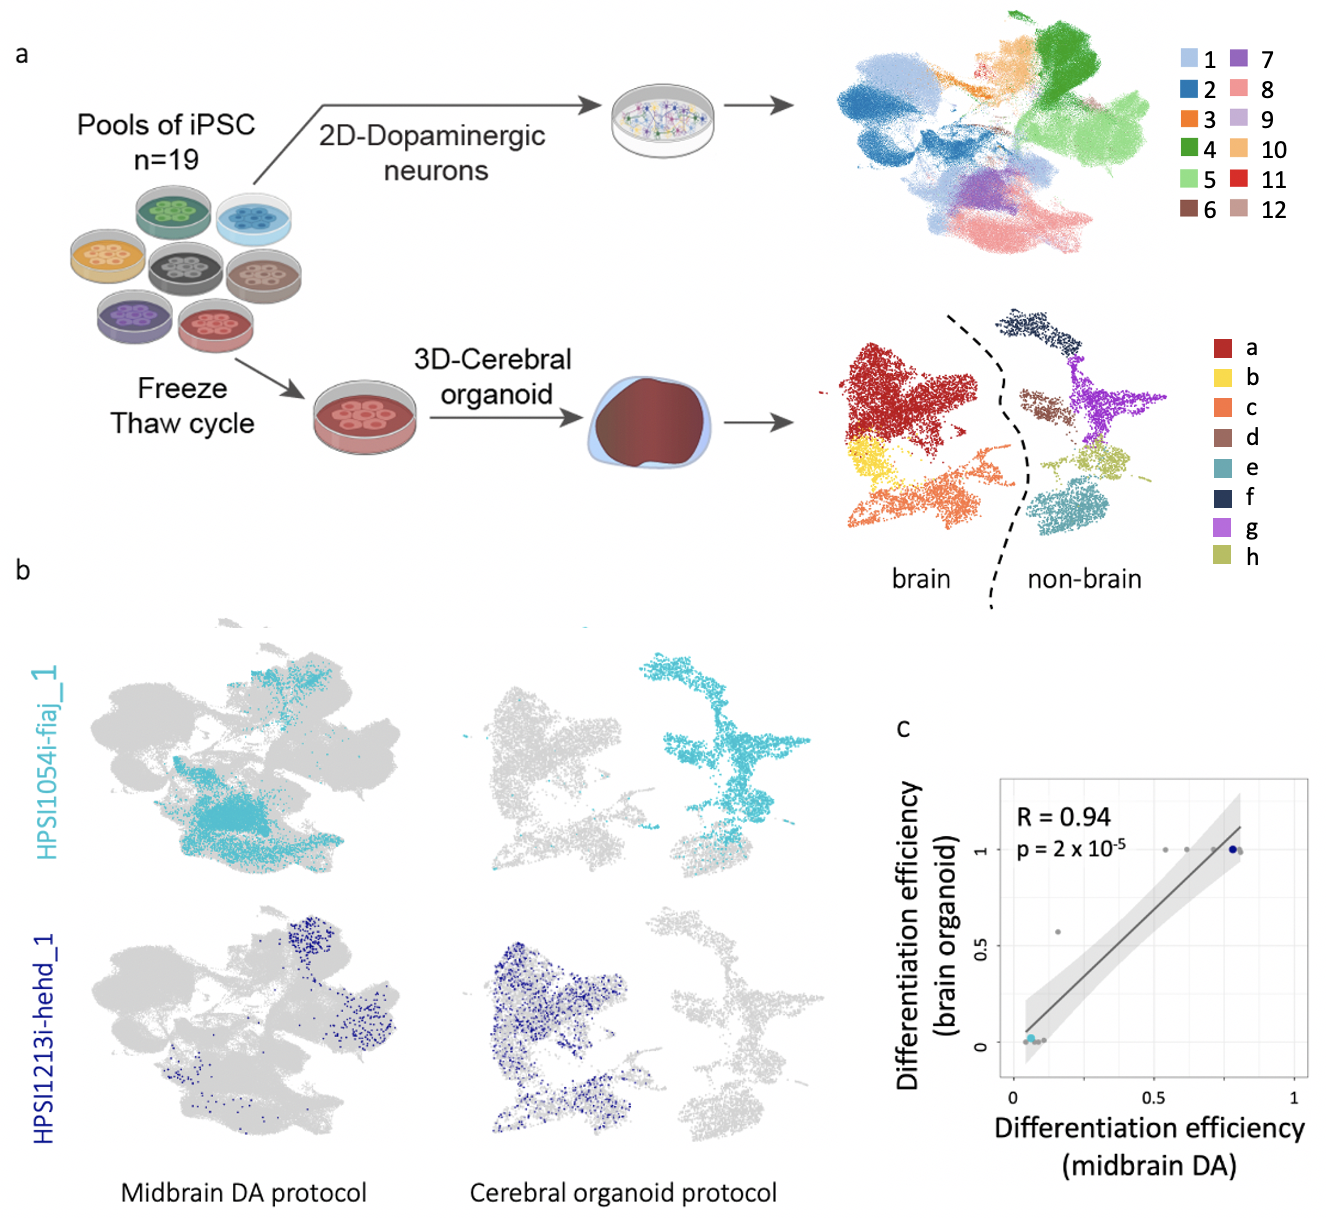
\includegraphics[width=11.5cm]{Chapter5/Fig/neuroseq_organoids.png}
\caption[Differentiation efficiency in cerebral organoids]{\textbf{Differentiation efficiency in cerebral organoids}.\\
(a) Experimental workflow for single cell profiling of iPSC-derived cerebral organoids using one pool containing 18 cell lines, profiled using scRNA-seq after 113 days of differentiation.
UMAPs for both our dopaminergic neuron study and the cerebral organoid study (1: floor plate progenitors (FPP), 2: proliferating FPP, 3: neuroblasts, 4: dopaminergic neurons (DA), 5: serotonergic-like neurons (Sert), 6: proliferating Sert, 7: astrocyte-like, 8: ependymal-like (Epen) 1, 9: Epen2, 10: unknown neurons (UN) 1, 11: UN2, 12: UN3.
a: neurons, b: intermediate progenitors, c: radial glial progenitors, d: satellite cells, e: mesenchymal cells, f: myotube, g: paired box (PAX)7+ cells, h: Wnt+ cells.)
(b) UMAPs of two representative cell lines making non-brain and brain cell types in the organoid study. 
(c) Scatter plot of neuronal differentiation efficiency as measured using midbrain dopaminergic neuronal differentiation (x axis) versus neural differentiation efficiency as measured in organoid differentiation (y axis) for a subset of 12 iPS cell lines in common. 
Highlighted are the same two cell lines as in (b).}
\label{fig:neuroseq_organoids}
\end{figure}

\clearpage

\section{iPSC expression can predict neuronal differentiation efficiency}
\label{sec:neuroseq_ips}

Motivated by the reproducibility of differentiation outcomes across multiple independent pools, we set out to explore possible predictors (similar to the analysis described in \textbf{section \ref{sec:endodiff_differentiation_efficiency}}).
The idea was that, if we could find characteristics that could be measured in iPSCs and that would predict a bad differentiation outcome, they could become a useful tool to select the most suitable lines prior to differentiation. \\

We began by testing for associations between neuronal differentiation efficiency and other experimental and biological factors.
Those included cell line passage number (p value = 0.77), donor sex (p value = 0.008), chromosome X activation status (p value = 0.01), and PluriTest scores \cite{muller2011bioinformatic} (p value = 0.01).
Although some of these were nominally significant, they explained little variation as compared to line-specific effects, when we performed variance component analysis, by modelling:

\begin{equation}\label{eq:neuroseq_vca}
    \mathrm{neuronal \ differentiation \ efficiency = Donor/Line + Pool + Sex + Age + \boldsymbol{\psi}},
\end{equation}

where Line (which cannot be distinguished from Donor), Pool, Sex and Age are all modeled as random effects (n=230 line-pool combinations).
To assess specifically the effect of X chromosome inactivation status, we fitted an alternative model which was limited to the female donors (n=115 line-pool combinations):

\begin{equation}\label{eq:neuroseq_vca_xci}
    \mathrm{neuronal \ differentiation \ efficiency = Donor/Line + Pool + XCI + Age + \boldsymbol{\psi}}. 
\end{equation}

\begin{figure}[htbp]
\centering
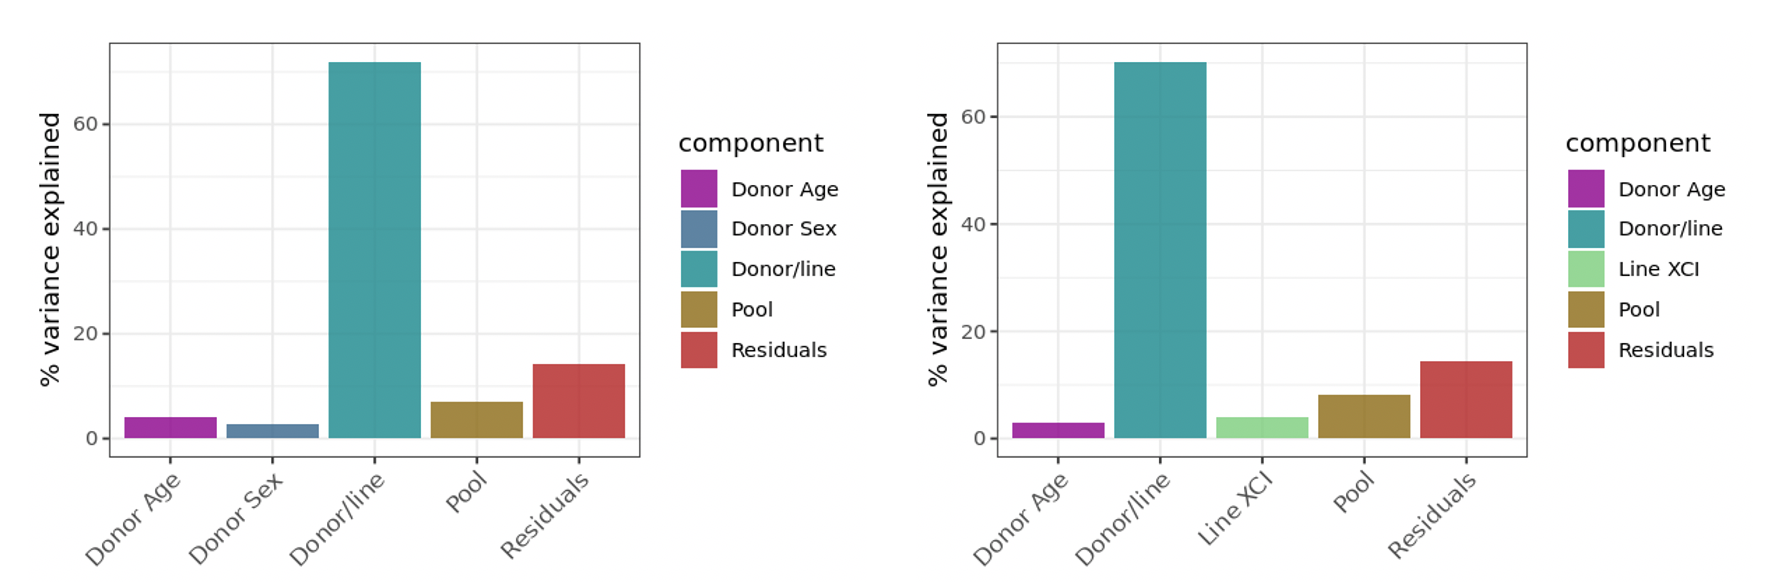
\includegraphics[width=16cm]{Chapter5/Fig/neuroseq_diff_eff_vca.png}
\caption[Variance component analysis of neuronal differentiation efficiency]{\textbf{Variance component analysis of neuronal differentiation efficiency}.\\
Results from variance component models in eq. \eqref{eq:neuroseq_vca} and \eqref{eq:neuroseq_vca_xci}, respectively.
The variance explained by each component was re-scaled to sum up to 100.
XCI is categorised into 0.1-wide bins: [0-0.1]..[0.4-0.5].}
\label{fig:neuroseq_diff_eff_vca}
\end{figure}

\newpage

We note that there is some effect of the technical batch iPSC lines were differentiated in, as it has been observed before \cite{kilpinen2017common, schwartzentruber2018molecular}, yet line-specific effects are prevalent (\textbf{Fig. \ref{fig:neuroseq_diff_eff_vca}}).
This is confirmed when we consider data from 6 lines (from pools 1, 2 and 3) that were differentiated individually, as well as in pools.
When we compared our measure of neuronal differentiation efficiency for each of the lines when differentiated alone or in a pool, we found rather concordant results (R = 0.83, p value = 0.034, n = 6).\\ 

Next, we assessed whether neuronal differentiation efficiency was associated with particular patterns of gene expression in undifferentiated iPSCs. 
Using data from independent bulk RNA-seq data available for a subset of 184 iPSC lines included in this study \cite{kilpinen2017common, bonder2019systematic} we identified significant associations with neuronal differentiation efficiency for 2,045 genes (983 positive and 1,062 negative associations; F-test, FDR < 5\%, \textbf{Fig. \ref{fig:neuroseq_ips_expression_signature}}). 

\begin{figure}[h]
\centering
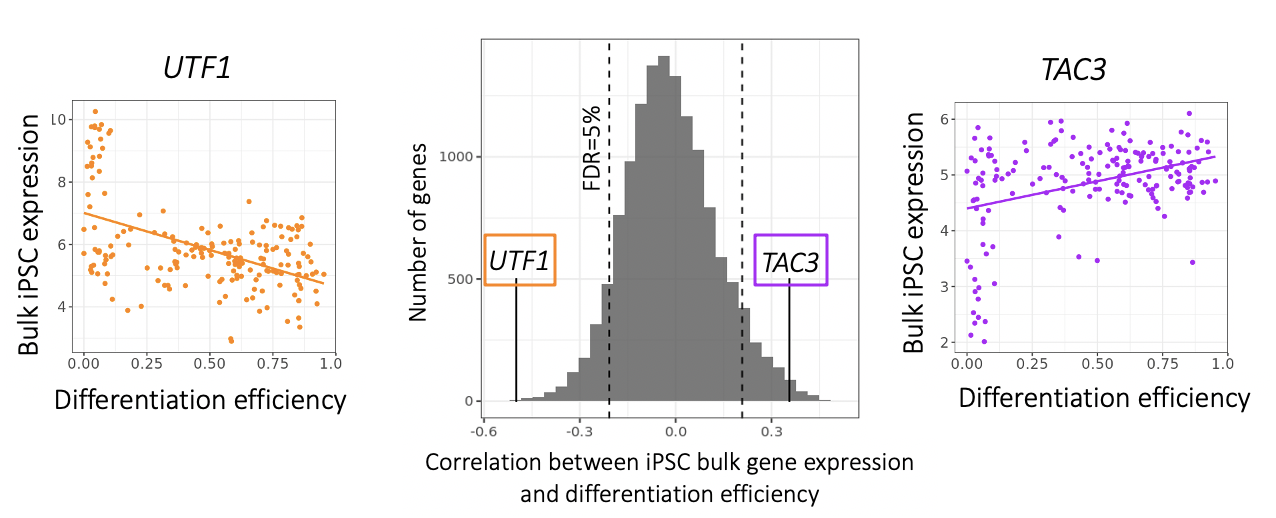
\includegraphics[width=16cm]{Chapter5/Fig/neuroseq_ips_bulk_expr_correlations.png}
\caption[iPS expression signature of neuronal differentiation efficiency]{\textbf{An iPSC expression signature is associated with neuronal differentiation efficiency}.\\
(middle) Histogram of Pearson correlation coefficients between iPSC gene expression of individual genes (measured using bulk RNA-seq \cite{bonder2019systematic}) and neuronal differentiation efficiency. 
Two exemplar genes (\textit{UTF1, TAC3}) are highlighted (left and right, respectively). 
\textit{UTF1} is an example of a gene whose expression level in iPSC (based on bulk RNA-seq) is negatively correlated with neuronal differentiation efficiency (R = -0.5, p value = 3.5$ \times 10^{-13}$ ), whereas \textit{TAC3} is positively correlated (R = 0.38, p value = 9.8$ \times 10^{-8}$).}
\label{fig:neuroseq_ips_expression_signature}
\end{figure}

\newpage

\subsection{A predictor of (poor) differentiation using iPSC gene expression}
\label{sec:neuro_diff_eff_predictor}

The examples shown in \textbf{Fig. \ref{fig:neuroseq_ips_expression_signature}} suggest that differentiation potential and especially poor differentiation (< 0.2) may be associated with clear expression signatures.
Motivated by this observation, we used the genome-wide gene expression signature in undifferentiated iPSCs to build a model to predict poor differentiation outcomes, where we defined poor differentiation as a binary outcome (neuronal differentiation efficiency < 0.2).
We used a logistic regression and obtained 100\% precision at 35\% recall as assessed by cross-validation. 
This result was robust to alternative thresholds for defining poor differentiation outcomes (\textbf{Fig. \ref{fig:neuroseq_diff_eff_predictor}}). 

\begin{figure}[h]
\centering
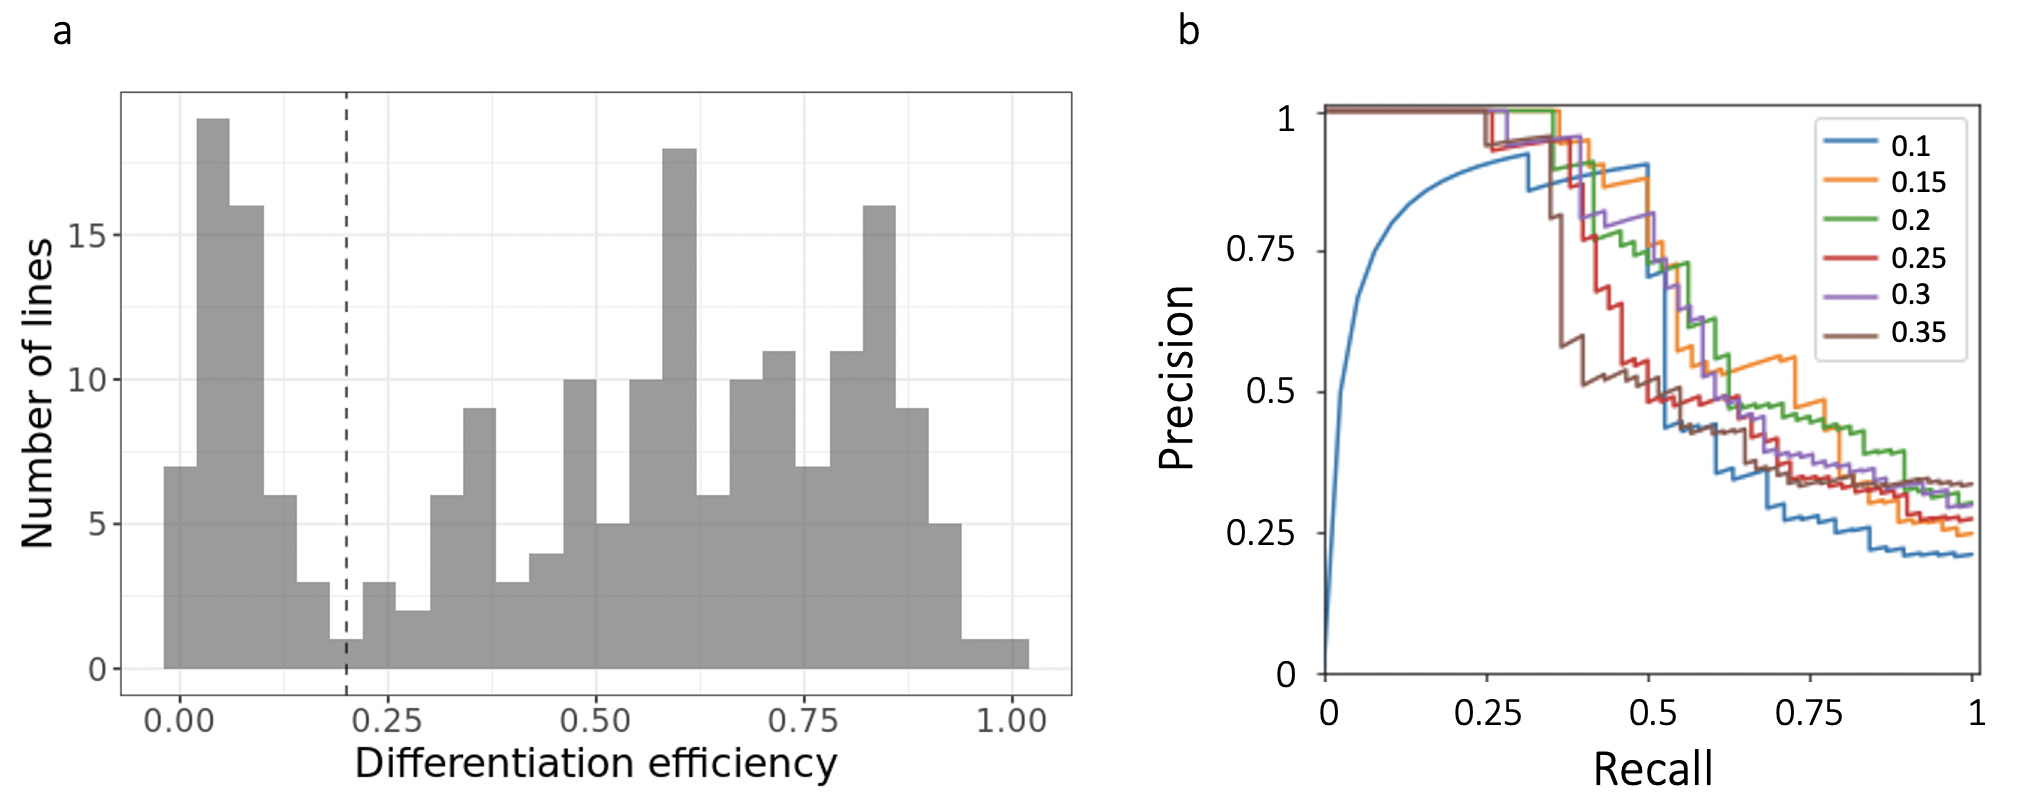
\includegraphics[width=15.5cm]{Chapter5/Fig/neuroseq_diff_eff_predict.png}
\caption[Predicting differentiation failure from iPSC gene expression]{\textbf{Predicting differentiation failure from iPSC gene expression}.\\
(a) Histogram of neuronal differentiation efficiencies across cell lines. 
The threshold chosen to define differentiation success or failure (i.e. neuronal differentiation efficiency = 0.2) is shown by the dashed line, separating the two modes of the distribution. 
(b) Precision-recall curves for a logistic regression model predicting differentiation failure from iPSC gene expression data \cite{bonder2019systematic} using a range of thresholds between 0.1 and 0.35 to define differentiation failure. 
Results are presented from leave-one-out cross validation.}
\label{fig:neuroseq_diff_eff_predictor}
\end{figure}

We then used this model to generate predicted scores for all 812 HipSci lines for which bulk RNA-seq data was available.
This analysis indicated that a substantial fraction of lines in the HipSci resource (26\%) were predicted to produce < 20\% neuronal cells under the differentiation conditions we tested.
Furthermore, we tested whether the same experimental and biological factors previously associated with neuronal differentiation efficiency replicated in this larger sample and found consistent results.
Finally, we did not observe strong concordance between the predicted differentiation outcomes of different cell lines from the same donor, suggesting that donor genetic background is unlikely to play an important role in driving differentiation biases (\textbf{Fig. \ref{suppl_fig:predicted_scores_donors}}).

\newpage

\subsection{A subpopulation of iPSCs is associated with poor differentiation}

Next, we hypothesised that the predictive gene expression signature identified in bulk RNA-seq at iPSC state may reflect variation in the proportion of subpopulations in iPSCs. 
To test this hypothesis, we re-analysed scRNA-seq data from 112 iPSC lines that were assayed previously under iPSC culture conditions similar to those used here \cite{cuomo2020single}, 45 of which were also included in this study\footnote{This is the day 0 population from the data presented in \textbf{Chapter \ref{chapter4}}, and the same iPSC single cell population used in \textbf{Chapter \ref{chapter3}}.}. 
After processing the data using the same pipeline as used above (i.e. Harmony batch correction, Louvain clustering),
we identified 5 clusters, which expressed similarly high levels of core pluripotency markers (\textit{NANOG, SOX2, POU5F1}, \textbf{Fig. \ref{fig:neuroseq_ips_sc_genes}, \ref{suppl_fig:ipsc_cluster2}}). \\

We found that genes whose expression predicted poor differentiation (e.g. \textit{UTF1}) were highly enriched in one of those clusters (cluster 2), while genes whose expression were predictive of successful differentiation (e.g. \textit{TAC3}), were downregulated in cluster 2 relative to the remaining iPSC clusters (\textbf{Fig. \ref{fig:neuroseq_ips_sc_genes}}). 
As a validation of this hypothesis, we also tested for and confirmed a significant association between the fraction of cells in cluster 2 and neuronal differentiation efficiency for each cell line (Pearson R = -0.76, p value = $2.05 \times 10^{-9}$, \textbf{Fig. \ref{fig:neuroseq_ips_sc_genes}}). 
We used additional data from \cite{cuomo2020single} to assess the consistency of the portion of cluster 2 cells across replication experiments, finding good concordance (Pearson R = 0.9; n=23, \textbf{Fig. \ref{fig:neuroseq_ips_sc_genes}}).
Using the known relationship between iPSC bulk RNA-seq and the proportion of cluster 2 cells, we predicted this proportion for 182 cell lines included in our differentiation experiments, and confirmed the negative correlation with neuronal differentiation efficiency (Pearson R = -0.49; p value = $3 \times 10^{-12}$, \textbf{Fig. \ref{suppl_fig:ipsc_cluster2}}). \\

\begin{figure}[htbp]
\centering
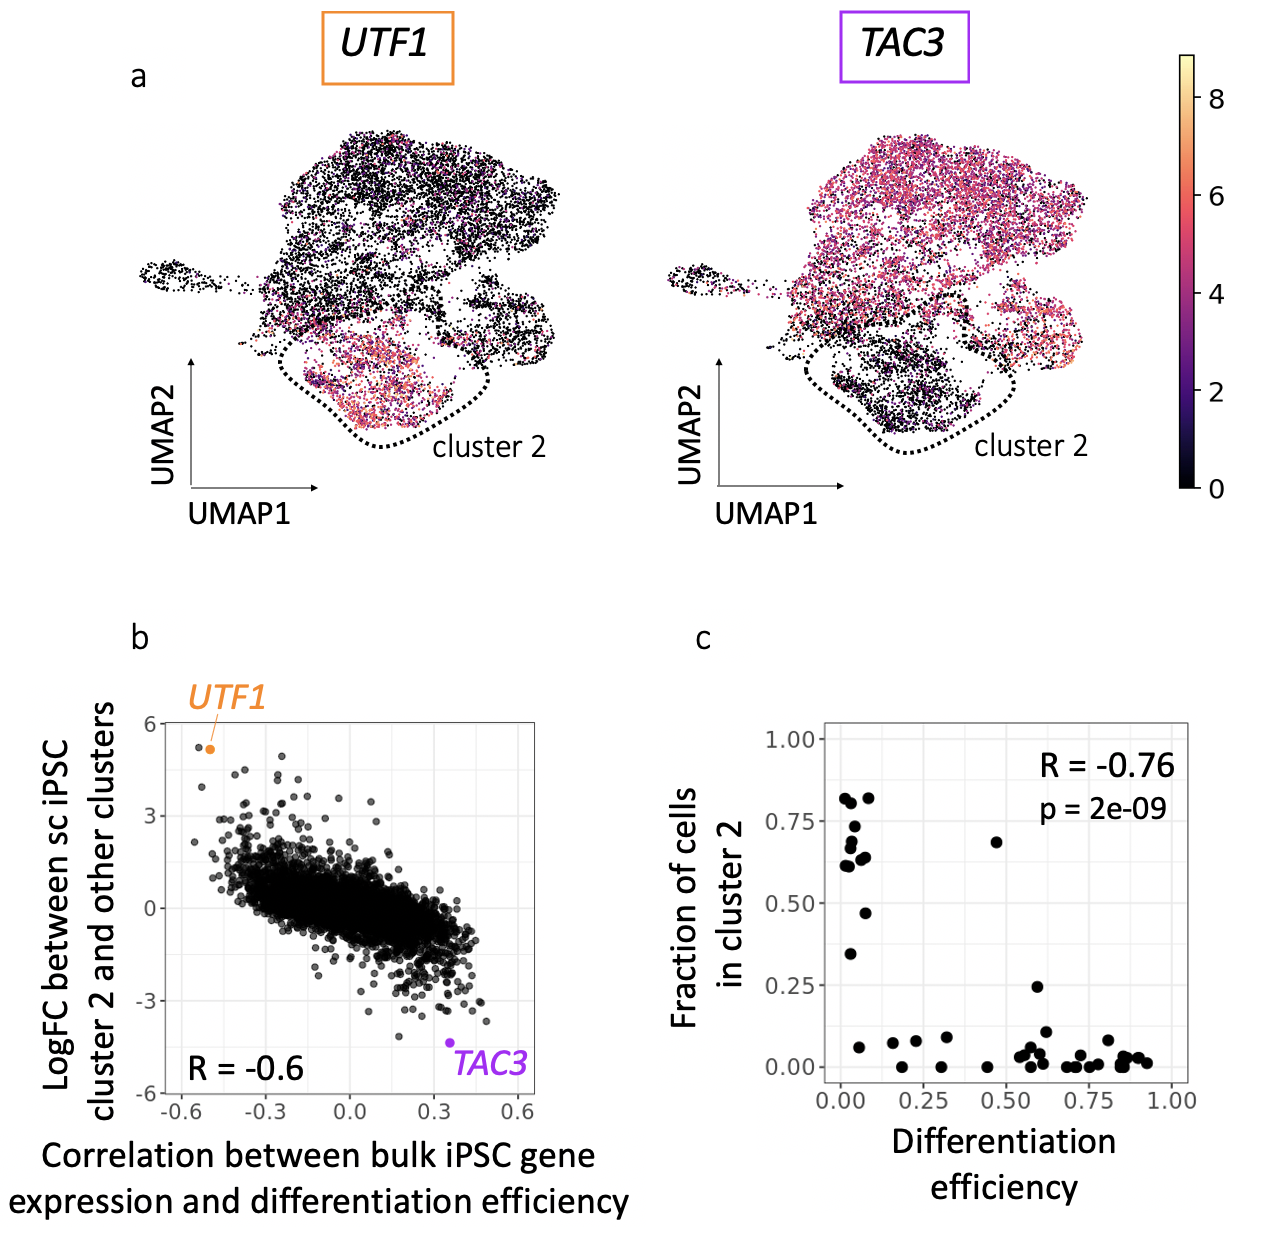
\includegraphics[width=14cm]{Chapter5/Fig/neuroseq_ips_sc_genes.png}
\caption[An iPSC subpopulation is linked to poor differentiation]{\textbf{A subpopulation of iPSCs is associated with poor differentiation}.\\
(a) UMAPs of single-cell RNA-seq profiles in iPSCs from 112 donors from \cite{cuomo2020single}.
Colours denote the expression level of the two example genes from \textbf{Fig. \ref{fig:neuroseq_ips_expression_signature}}: \textit{UTF1} and \textit{TAC3}. 
Cluster 2 is shown by the dashed lines. 
(b) Comparison of marker gene association results with expression markers of the cluster 2. 
For each gene, the Pearson correlation coefficient of association between the gene's iPSC expression and neuronal differentiation efficiency (x axis; iPSC gene expression assessed using bulk RNA-seq, as in \textbf{Fig. \ref{fig:neuroseq_ips_expression_signature}}) is compared to its log fold change between cluster 2 and all other clusters (y axis, scRNA-seq).
\textit{UTF1}, and \textit{TAC3} are highlighted. 
(c) Scatter plot between the proportion of cells assigned to cluster 2 (y axis) and neuronal differentiation efficiency (x axis) across 45 cell lines which were included in both sets of experiments. 
Where measurements across multiple pools were available for a cell line, these were averaged.}
\label{fig:neuroseq_ips_sc_genes}
\end{figure}

Finally, we also analysed an additional scRNA-seq dataset from iPSCs derived from Lymphoblastoid Cell Lines (LCLs) \cite{sarkar2019discovery}. 
Using our single cell analysis pipeline, we identified a cluster of cells with a concordant ($R^2$=0.4) expression profile to cluster 2 (\textbf{Fig. \ref{suppl_fig:ipsc_cluster2_sarkar}}). 
Combined, these results provide further evidence that an iPSC sub-population with poor differentiation capability can be consistently detected across iPSCs from different banks, and that this bias can be predicted robustly using gene expression at iPSC stage. \\

Importantly, despite the variability in neuronal differentiation efficiencies, 
we still retained significant numbers of cells across many cell lines and disease-relevant cell types and stimuli, which enabled us to explore the impact of common genetic variants on gene expression, across such cell populations (next section, \textbf{section \ref{sec:neuroseq_eqt}}).

\newpage

\section{Mapping eQTL in neuronal cell types}
\label{sec:neuroseq_eqt}

Next, in order to understand how individual-to-individual genetic variation influenced gene expression in this system, we mapped \glspl{eqtl} across our identified cell types during differentiation, and in response to stimulation.
Specifically, we mapped \textit{cis} \gls{eqtl} in each of the well represented\footnote{top 4 cell types per condition with at least 20\% cells.} `cell type'-`condition' contexts defined above i.e. the 14 distinct cell populations shown in \textbf{Table \ref{tab:eqtl_maps}}. 

\begin{table}[h]
    \centering
    \begin{tabular}{c|c c c c c c}
    &         FPP & P\_FPP & DA & Sert & Epen1 & Astro \\
    \hline
    Day 11  &  \checkmark & \checkmark   \\
    Day 30  & \checkmark & & \checkmark & \checkmark & \checkmark  \\
    Day 52 - untreated & & & \checkmark & \checkmark & \checkmark & \checkmark \\
    Day 52 - ROT treated & & & \checkmark & \checkmark & \checkmark & \checkmark \\
    \end{tabular}
    \caption[Overview of eQTL maps]{Overview of the 14 cell populations we mapped eQTL for (rows: conditions, columns: cell types).
    FPP: floor plate progenitors; P\_FPP: proliferating FPP; DA: dopaminergic neurons; Sert: serotonergic-like neurons; Epen1: ependymal-like cell population 1; Astro: astrocyte-like.}
    \label{tab:eqtl_maps}
\end{table}

\textit{Cis} \gls{eqtl} were mapped by calculating average expression levels for each donor\footnote{Similar to the d-mean aggregation method described in \textbf{Chapter \ref{chapter3}, section \ref{sec:best_practice}}.}, considering common gene-proximal variants (MAF > 0.05, +/- 250 kb around genes). 
For each context (cell type, condition), all genes detected in at least 1\% of the cells of that context
were tested, and expression quantification was only included for a donor if it represented the mean of at least 10 cells. 
The observed variability in neuronal differentiation efficiency between lines\footnote{i.e. as we have seen, some lines made mostly neuronal cell types and barely any non-neuronal, thus expression estimates for those lines in non-neuronal cell types will be less accurate because they are estimated using very few cells, and vice versa for lines that mostly made non-neurons, and very few neurons.} (\textbf{Fig. \ref{fig:neuroseq_diff_efficiency}}) resulted in substantial differences in the number of cells collected for each donor, affecting accuracy of the estimates of aggregated expression. 
To account for this source of noise, we adapted commonly used \gls{eqtl} mapping strategies \cite{cuomo2020single} based on LMMs (\textbf{Chapter \ref{chapter2}}) by incorporating an additional variance component into the model:

\begin{equation}\label{eq:neuroseq_ncell}
    \mathbf{y} = \sum_i^{15}\alpha_i \mathbf{PC}_i + \mathbf{g}\beta + \tilde{\mathbf{u}} + \boldsymbol{\psi}, 
\end{equation}

where $\tilde{\mathbf{u}} \sim \mathcal{N}(\mathbf{0}, diag(\frac{1}{n_i}))$, where $n_i$ is the number of cells for each individual i.
Note that since our LMM implementation only allows one random effect component to be considered (see\textbf{ page \pageref{sec:non_gaussian}}), in this model we are not accounting for population structure.
Consequently, we have to rely on samples being unrelated (\textbf{Fig. \ref{suppl_fig:no_pop_struct}}), and cannot consider multiple observations for the same lines (e.g. across pools). 
Therefore, expression was aggregated at the cell line/donor level, averaged across pools for the lines assessed in more than one pool. 
Using this approach, we found
a total of 4,828 genes with at least one \gls{eqtl} in any of the contexts (hereafter `eGenes', FDR < 5\%, Storey procedure, \textbf{Table \ref{tab:eqtl_results}}).

\begin{table}[h]
    \centering
    \begin{tabular}{c|c c c c c c}
    &         FPP & P\_FPP & DA & Sert & Epen1 & Astro \\
    \hline
    Day 11  & 2,560 & 2,457 & - & - & - & - \\
    Day 30  & 881 & - &  872 & 776 & 1,011 & -  \\
    Day 52 - untreated & - & - & 1,024 & 1,436 & 1,391 & 257 \\
    Day 52 - ROT treated & - & -  & 458 & 1,043 & 1,122 & 205 \\
    \end{tabular}
    \caption[Number of eGenes across contexts]{Number of eGenes at FDR < 5\% for each assessed eQTL map.
    FPP: floor plate progenitors; P\_FPP: proliferating FPP; DA: dopaminergic neurons; Sert: serotonergic-like neurons; Epen1: ependymal-like cell population 1; Astro: astrocyte-like.}
    \label{tab:eqtl_results}
\end{table}

This approach greatly increased the number of detected \gls{eqtl}, as compared to the base-model which does not include the noise term, i.e.:

\begin{equation}\label{eq:neuroseq_base}
    \mathbf{y} = \sum_i^{15}\alpha_i \mathbf{PC}_i + \mathbf{g}\beta + \boldsymbol{\psi},
\end{equation}

confirming the importance of taking into account the large effect that the number of cells for each individual has on the uncertainty of the mean expression estimation (\textbf{Fig. \ref{fig:neuroseq_eqtl_improved_power}}). 

\begin{SCfigure}[1][!h]
\caption[Increase in number of discovered eQTL]{\textbf{Increase in number of discovered eQTL}.
Number of eGenes for each cell type, time point and stimulation discovered using either a traditional linear model (coral, from eq. \eqref{eq:neuroseq_base}) or our enhanced model accounting for noise due to variation in the number of cells collected for each donor (seagreen, from eq. \eqref{eq:neuroseq_ncell}).
FPP: floor plate progenitors; P\_FPP: proliferating FPP; DA: dopaminergic neurons; Sert: serotonergic-like neurons; Epen1: ependymal-like cell population 1; Astro: astrocyte-like}
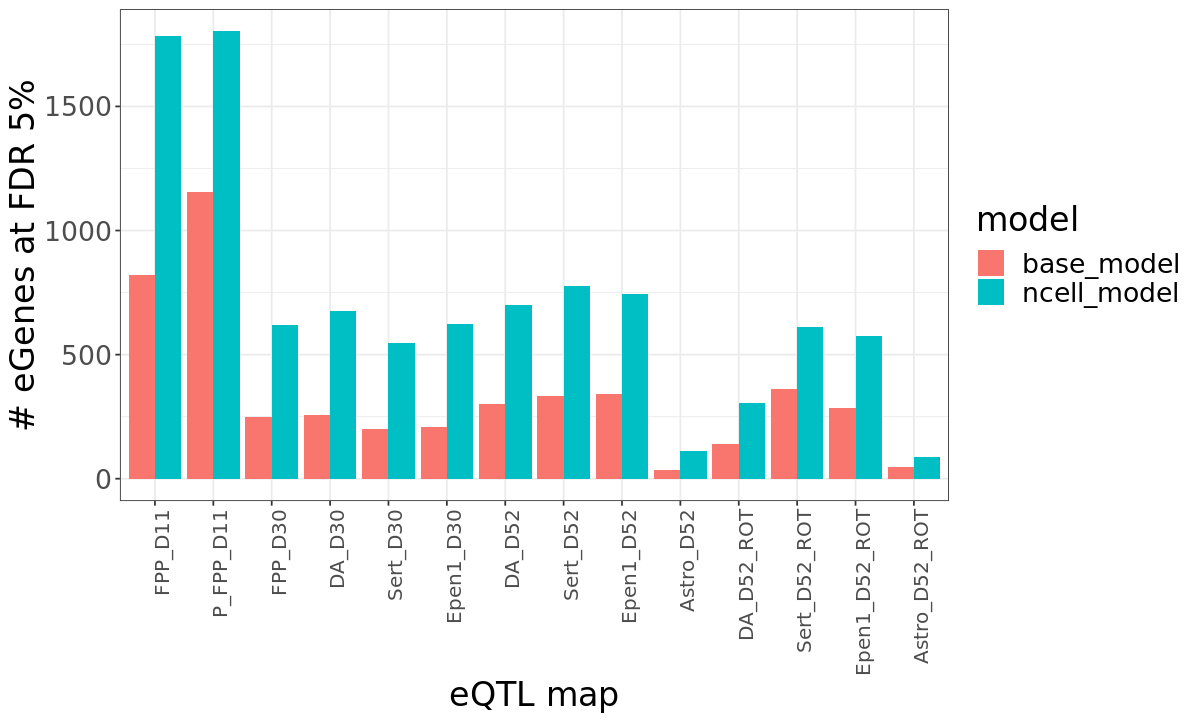
\includegraphics[width=0.7\textwidth]{Chapter5/Fig/neuroseq_improved_eqtl_power.png}
\label{fig:neuroseq_eqtl_improved_power}
\end{SCfigure}

\newpage

The main insight from this specific analysis is that variation in cell count across donors for a given cell type/condition (\textbf{Fig. \ref{fig:neuroseq_line_variation},\ref{fig:neuroseq_diff_efficiency}}) is a substantial source of variation in single-cell based designs. 
Accounting for this effect in the noise model substantially improves the ability to detect eQTL (\textbf{Fig. \ref{fig:neuroseq_eqtl_improved_power}}).
This is especially pronounced in this dataset, and motivated us to prioritise accounting for this source of variability over considering data across multiple batches (i.e. dr-mean, which had emerged as the best approach in \textbf{Chapter \ref{chapter3}, section \ref{sec:best_practice}}).

\subsection{Comparison with alternative eQTL methods}
\label{sec:neuroseq_eqtl_methods}

In order to more generally compare alternative approaches to map eQTL, for one selected cell population (untreated dopaminergic neurons at day 52), we compared our results (which yelded 1,024 eGenes, \textbf{Table \ref{tab:eqtl_results}}) to those obtained from alternative eQTL methods.
Specifically, these methods differ in the approach taken to account for variability in cell count (or not), and in how we deal with replicate lines in the analysis.
In particular, by aggregating at the donor level, we may not be accounting properly for batch differences.
As an alternative, we could aggregate at the line and experiment level (similar to the dr-mean approach described in \textbf{Chapter \ref{chapter3}}, which is also adopted in the eQTL analysis from \textbf{Chapter \ref{chapter4}}), and use a standard kinship matrix-approach to account for the repeatedness (rather than the number of cells noise term), i.e. test the following model:

\begin{equation}\label{eq:neuroseq_pcs_kinship}
    \mathbf{y} = \sum_i^{15}\alpha_i \mathbf{PC}_i + \mathbf{g}\beta + \mathbf{u} + \boldsymbol{\psi}, 
\end{equation}
where $ \mathbf{u} \sim \mathcal{N}(\mathbf{0},\sigma_g^2\mathbf{K})$;
In this model, we do not account for the variability in cell count; this resulted in 471 eGenes at FDR < 5\%.
Another possibility would be to include the batch (and sex) directly as (several) covariates, such that:

\begin{equation}\label{eq:neuroseq_batch_kinship}
    \mathbf{y} = \sum_i^{16}\alpha_i \mathbf{pool}_i + 
    \gamma \ \mathbf{sex} + 
    \mathbf{g}\beta + \mathbf{u} + \boldsymbol{\psi}, 
\end{equation}

where $ \mathbf{u} \sim \mathcal{N}(\mathbf{0},\sigma_g^2\mathbf{K})$.
This resulted in markedly fewer eGenes - 320.
Finally, in order to account for batch effects whilst still including the number-of-cell noise term, it is possible to only consider one experiment per line, and correct for pool, as well as sex, as covariates:

\begin{equation}\label{eq:neuroseq_batch_ncell}
    \mathbf{y} = \sum_i^{16}\alpha_i \mathbf{pool}_i + \gamma \ \mathbf{sex} + \mathbf{g}\beta + \tilde{\mathbf{u}} + \boldsymbol{\psi}, 
\end{equation}

where $\tilde{\mathbf{u}} \sim \mathcal{N}(\mathbf{0}, diag(\frac{1}{n_i}))$, and $n_i$ is the number of cells for each individual i, as above.
This approach, too, resulted in fewer eGenes (608) compared to our chosen approach.

\begin{figure}[htbp]
\centering
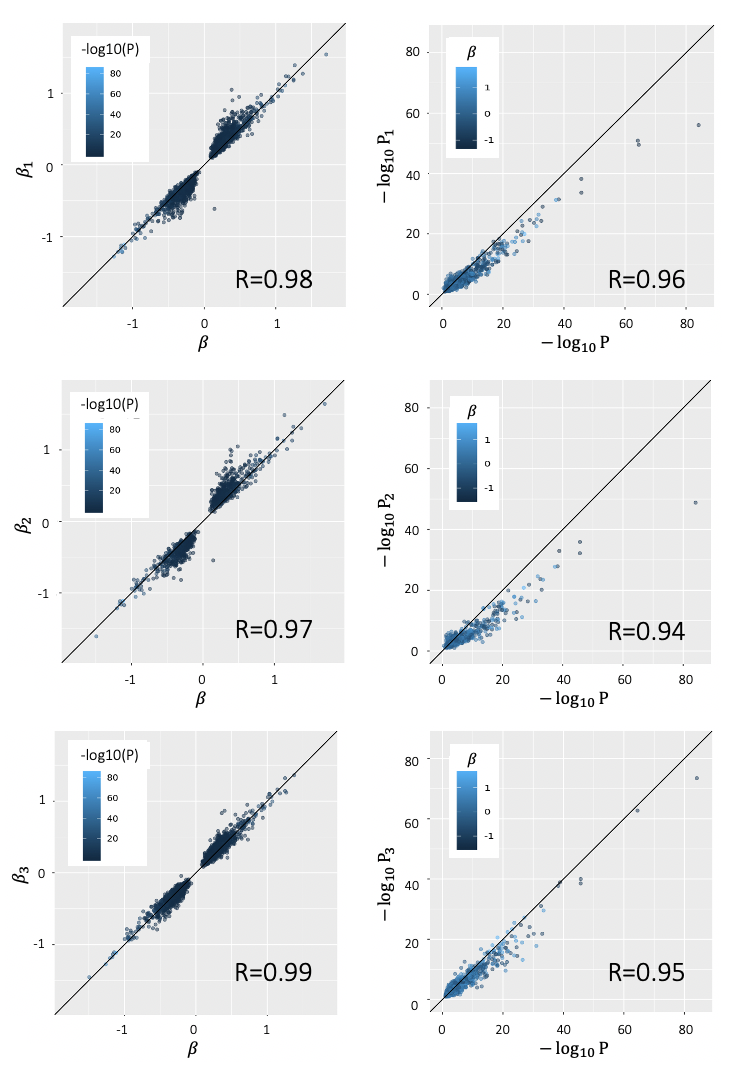
\includegraphics[width=13.5cm]{Chapter5/Fig/neuroseq_eqtl_methods_corr.png}
\caption[eQTL methods comparison]{\textbf{eQTL methods comparison}.\\
Scatter plots of \gls{eqtl} effect sizes (left) and p values (right) obtained when testing association of untreated day 52 dopaminergic neuron \gls{eqtl} discovered using our approach (from eq. \eqref{eq:neuroseq_ncell}, x axis) and each of the three alternative methods described in equations \eqref{eq:neuroseq_pcs_kinship}, \eqref{eq:neuroseq_batch_kinship} and \eqref{eq:neuroseq_batch_ncell}, respectively (y axis). 
Pearson's correlations (R) are indicated.}
\label{fig:neuroseq_eqtl_methods_comp}
\end{figure}


Compared to these alternative methods, our approach resulted in the most discoveries (with 1,024 eGenes, see \textbf{Table \ref{tab:eqtl_results}}), yet the results were highly consistent between methods (\textbf{Fig. \ref{fig:neuroseq_eqtl_methods_comp}}), excluding the possibility that our model may be generating mostly false positives.
This demonstrates that our results are robust to these specific choices, with the strategy we chose yielding more total eQTL discoveries. 
As an additional quality control metric, frequently used by other studies (e.g. \cite{gtex2015genotype}), we assess and confirm an enrichment of eQTL variants at gene promoters (\textbf{Fig. \ref{fig:neuroseq_eqtl_TSS}}).

\begin{figure}[h]
\centering
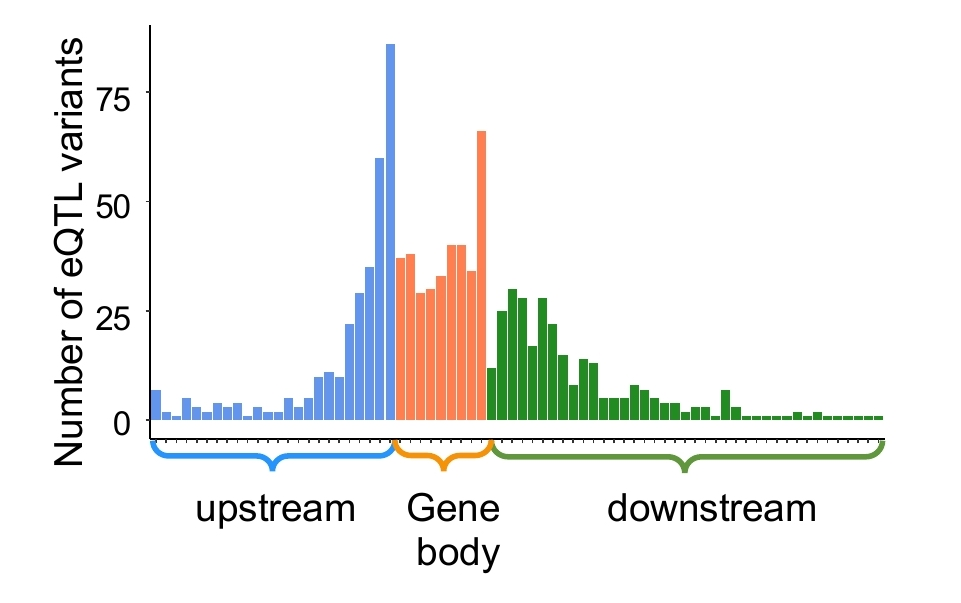
\includegraphics[width=12cm]{Chapter5/Fig/TSS_distr.jpg}
\caption[Distribution of eQTL genomic locations]{\textbf{Distribution of eQTL genomic locations}.\\
Genomic location of eQTL lead variants relative to normalised gene coordinates, considering 1,024 eQTL identified in day 52 untreated dopaminergic neurons (using eq. \eqref{eq:neuroseq_ncell}).}
\label{fig:neuroseq_eqtl_TSS}
\end{figure}

Moreover, the incorporation of PCs is an efficient approach for capturing global trends and hence can often replace the use of a potentially large number of technical covariates (e.g. we have 16 pools in our data alone).
Additionally, accounting for pool is not straightforward in our study, as some lines (n=35) were included in two pools. 
Finally, we have also tested the extent to which the 15 PCs we have included in our model capture the key known covariates, which we do not model directly. 
When fitting a linear model to explain different covariates as a function of the 15 PCs:

\begin{equation}
    \mathbf{cov} = \mathbf{PC}_1 + .. + \mathbf{PC}_{15} + \boldsymbol{\epsilon},
\end{equation}

We observed that the 15 PCs explained 57\% of the variance across pools (where only one pool replicate was considered for lines differentiated in multiple pools), 67\% of the variance of the donor sex covariate (male=0, female=1), 78\% of the X chromosome status, and 9\% of average age.

\clearpage

\subsection{Comparison of eQTL across cell types and conditions}

Next, we set out to compare eQTL maps across cell types and conditions.
First, we observed that the largest number of \gls{eqtl} were detected in progenitor cell populations, likely reflecting increased detection power due to the larger number of well-represented donors (> 100 cells per donor). 
Next, we noted that the cumulative number of eGenes (genes with an \gls{eqtl}) in each cell type increased considerably when taking into account cells further progressed along the differentiation axis, as well as upon stimulation (\textbf{Fig. \ref{fig:neuroseq_eqtl}}). 


\begin{figure}[h]
\centering
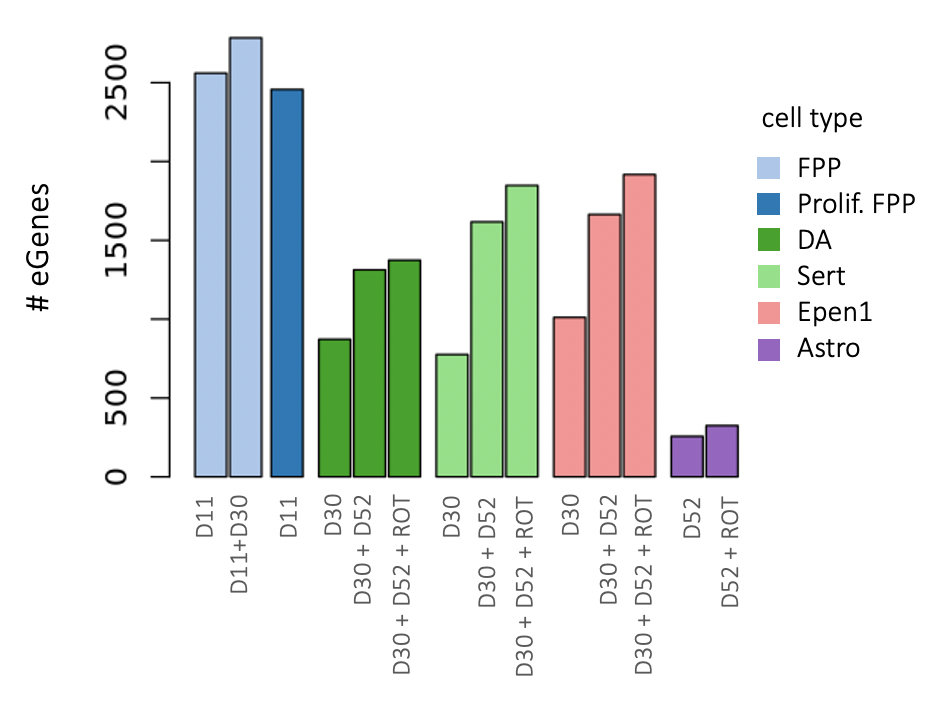
\includegraphics[width=14cm]{Chapter5/Fig/neuroseq_eqtl_cumulative.png}
\caption[Mapping eQTL across neuronal cell types]{\textbf{Mapping \textit{cis} eQTL in distinct cell contexts across midbrain differentiation}.\\
Cumulative number of eGenes for each cell type and condition (D11 = day 11; D30 = day 30; D52 = day 52 (untreated); ROT = rotenone-treated day 52).}
\label{fig:neuroseq_eqtl}
\end{figure}

For example, in DA cells, eQTL mapping in matured (untreated) cells (day 52) identified an additional set of 441 eGenes (at FDR < 5\%) compared to day 30 cells.
An example of a timepoint-specific eGene is \textit{HSPB1}, for which SNP rs6465098 is an eQTL in day 52 cells, but not day 30 (\textbf{Fig. \ref{fig:neuroseq_eqtl_examples}}). 
\textit{HSPB1} encodes a heat shock protein that plays a key role in neuronal differentiation \cite{miller2018heat} and for which changes in gene expression have been observed in neurons after ischemia \cite{bartelt2016hspb5} and associated with toxic protein accumulation in Alzheimer's disease \cite{shimura2004binding, wilhelmus2006small}.\\

Similarly, we detected 248 additional eGenes with a rotenone-specific effect in DA and Sert neurons. 
As an example, the SNP variant rs12597281 is an eQTL for \textit{ACSF3} in rotenone-stimulated serotonergic-like neurons at day 52, but not in unstimulated cells (\textbf{Fig. \ref{fig:neuroseq_eqtl_examples}}). 
\textit{ACSF3} encodes an acyl-CoA synthetase localised in the mitochondria and for which inherited mutations have been associated with a metabolic disorder, combined malonic and methylmalonic aciduria (CMAMMA), where patients exhibits a wide range of neurological symptoms including memory problems, psychiatric problems and/or cognitive decline \cite{tucci2020brain}.\\

These examples highlight how changes in the expression of genes known to be associated with human disease can be transient and specific to a cell type and state. 
More importantly, this data shows how our experimental design brings an extra level of resolution to understand disease mechanisms that were previously inaccessible from primary tissues, and opens up new experimental avenues. \\


\begin{figure}[h]
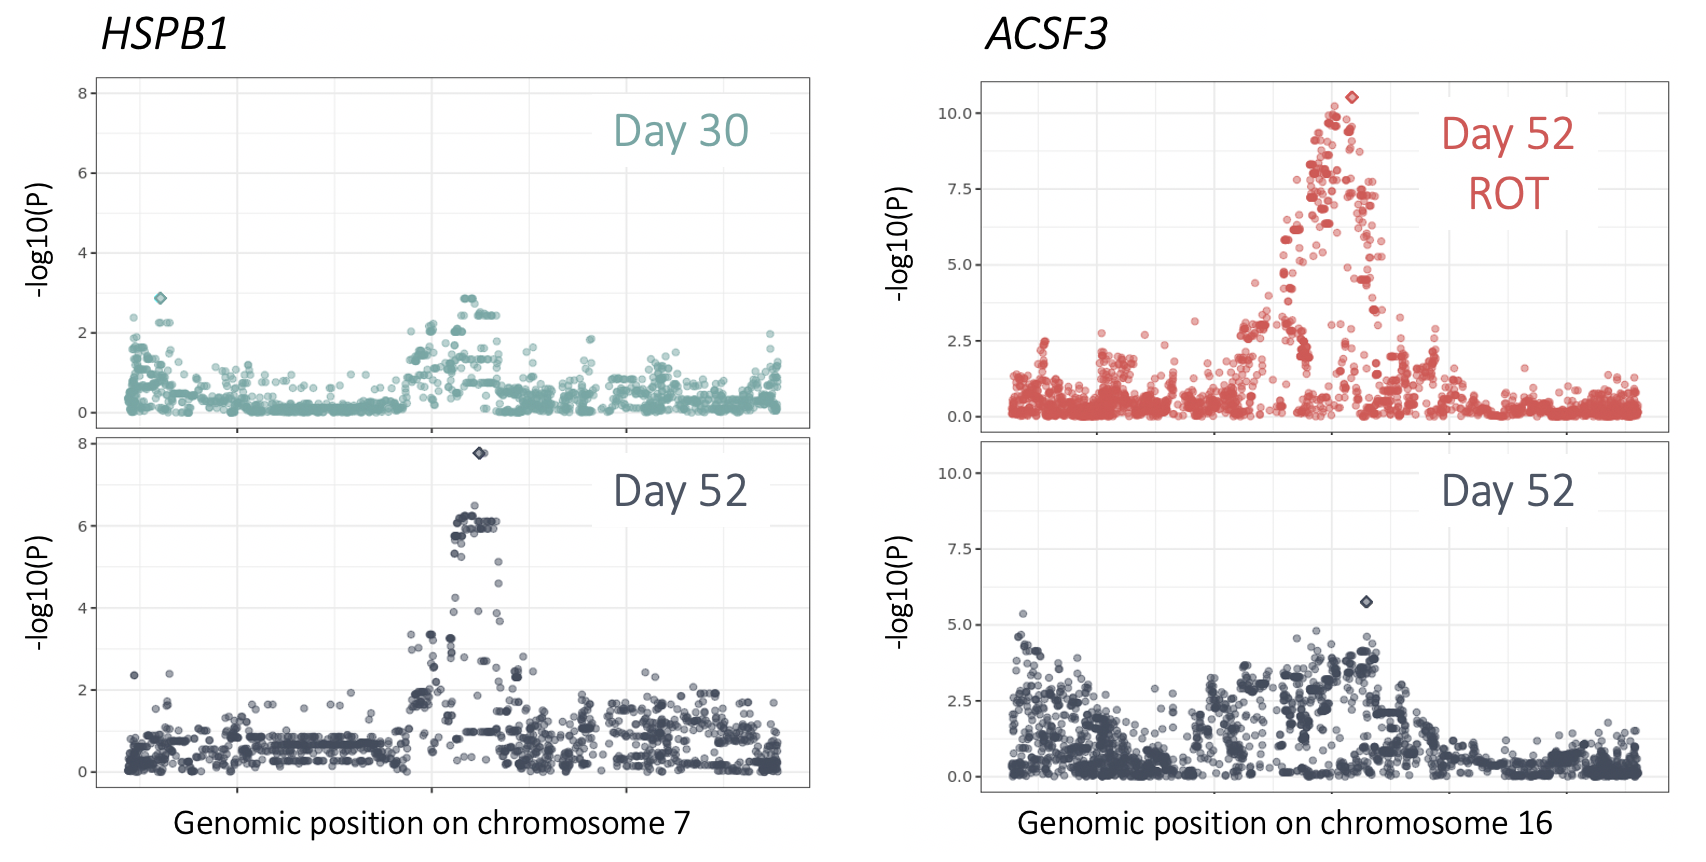
\includegraphics[width=16cm]{Chapter5/Fig/neuroseq_eqtl_examples.png}
\caption[Context-specific eQTL examples]{\textbf{Context-specific eQTL examples}.\\
Left: day 52-specific eQTL for \textit{HSPB1} in DA (rs6465098; FDR < 5\%). 
In figure are Manhattan plots for DA cells at day 30 (top) and day 52 (bottom). 
Right: a rotenone stimulus-specific eQTL for \textit{ACSF3} in serotonergic-like neuronal cells (rs12597281, right). 
Manhattan plots are shown for rotenone-stimulated (top) and unstimulated (bottom) Sert day 52 cells.}
\label{fig:neuroseq_eqtl_examples}
\end{figure}

\clearpage

\subsection{Comparison of eQTL from our study with \textit{in vivo} maps}

In order to put our eGene discovery in relation to previous studies, we compared the number of eGenes identified here with bulk eQTL maps from \textit{in vivo} tissues from the GTEx consortium \cite{gtex2017genetic}. 
For a first coarse-grain comparison between bulk and single-cell eQTL maps,
we aggregated\footnote{Considered the union of eQTL identified in any of our 14 cell populations.} eQTL across cell types and found that the number of discovered eGenes was similar to that expected in a primary tissue of the same sample size (\textbf{Fig. \ref{fig:neuroseq_and_gtex_power}}). \\

However, when focusing on individual cell populations, we observed fewer `cell type'-`condition' eGenes than detected in GTEx tissues of similar sample size (\textbf{Fig. \ref{fig:neuroseq_and_gtex_power}}), likely due to the uneven representation of donors across cells, which in turn results in noisier expression estimates compared to the GTEx results using bulk measurements.
This result is consistent with what we observed in work presented in \textbf{Chapter \ref{chapter3}}, where we found increased number of discoveries when mapping eQTL using bulk compared to single cell RNA-seq, even when considering the same cell type and matched individuals. 

\vspace{2mm}

\begin{figure}[h]
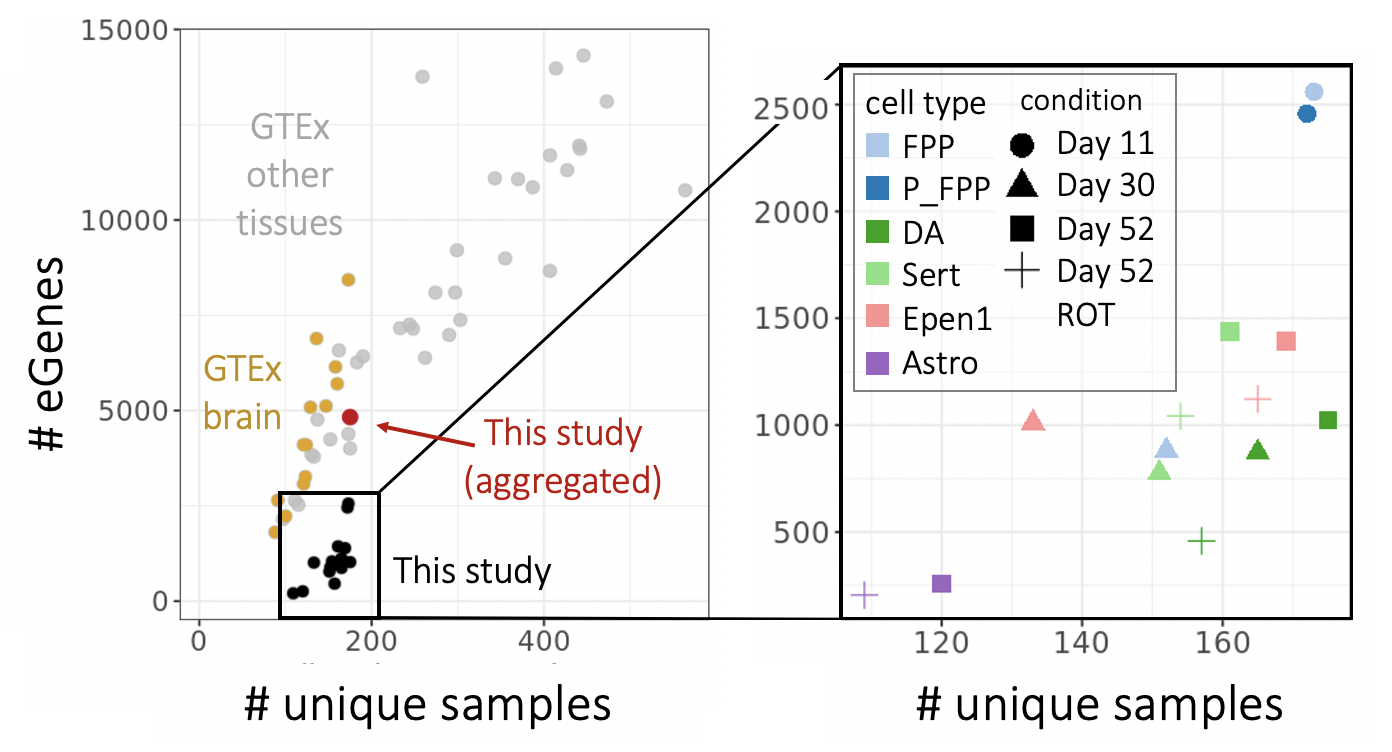
\includegraphics[width=13cm]{Chapter5/Fig/neuroseq_eqtl_gtex_scatterplot.png}
\caption[Sample size vs number of discoveries]{\textbf{Sample size vs number of discoveries}.\\
Comparison of the number of genes with at least one eQTL (number of eGenes; FDR < 5\%; y axis) as a function of effective sample size (number of unique donors; x axis) across studies and cell types. 
Left: results from overlapping eQTL results in this study with \textit{in vivo} eQTL maps from GTEx, divided into brain tissues and non-brain tissues. 
The result from our study when aggregating across cell types and conditions is coloured in red. 
The right panel shows a magnified view of results from our study coloured by cell type and shaped by condition.
Astro: Astrocyte-like, DA: Midbrain dopaminergic neurons, Epen1: Ependymal-like, FPP: Floor Plate Progenitors, P\_FPP: Proliferating FPP, Sert: Serotonergic-like neurons.
ROT: rotenone-treated.}
\label{fig:neuroseq_and_gtex_power}
\end{figure}

\newpage

A key question of eQTL maps from \textit{in vitro} iPSC-based models is how closely these resemble eQTL maps from the equivalent primary tissues, which typically differ in cell type composition. 
To explore this, we tested the extent to which regulatory variants were shared between our eQTL maps and 48 \textit{in vivo} maps from the GTEx consortium, as measured by genome-wide consistency of eQTL effect sizes (using MASHR \cite{urbut2019flexible}).
First, reassuringly, we observed that the sharing of genetic signal\footnote{Following recommendations by the MASHR authors \cite{stephens2020eqtl}, for each pair of conditions, we considered eQTL that were significant (local false sign rate < 0.05) in at least one of the two conditions, and then assessed sharing as the fraction of those for which posterior estimates of effect size were of similar magnitude ($0.5 <$ ratio $<2$) and of concordant direction of effect.} between our eQTL maps and GTEx tissues is considerably higher when we consider brain tissues compared to all other tissues 
(using the subset of 6,205 genes that were assessed in each of our cell types and in all GTEx tissues; \textbf{Fig. \ref{fig:neuroseq_and_gtex_brain_sharing}}, panel a). \\

Next, we performed a second MASHR analysis, this time including only the 13 GTEx brain tissues (as well as our 14 maps, and one iPSC map from \cite{bonder2019systematic}). 
The main motivation to do so is that in order to quantify the amount of sharing between eQTL results obtained from several tissues or conditions, MASHR only considers gene-SNP pairs that have been assessed in every one of the conditions considered, which naturally will depend on the number of genes expressed in the various conditions and that can be quantified by the different technologies used. \\

As a consequence, the number of genes considered decreases as the number of conditions included increases, which in turn results in the inflation of the amount of sharing.
Here, in particular, excluding non-brain eQTL maps from GTEx rescued several brain-specific genes, and allowed us to assess sharing for 8,706 genes ($\sim$2,500 more).
This second analysis enabled us to assess the similarity of our maps to the brain tissues in particular. 
We found that the extent of eQTL sharing between our eQTL maps and GTEx brain tissues increased as iPSCs were differentiated to increasingly mature neuronal cell types (\textbf{Fig. \ref{fig:neuroseq_and_gtex_brain_sharing}}, panel b). 

\begin{figure}[h]
\centering
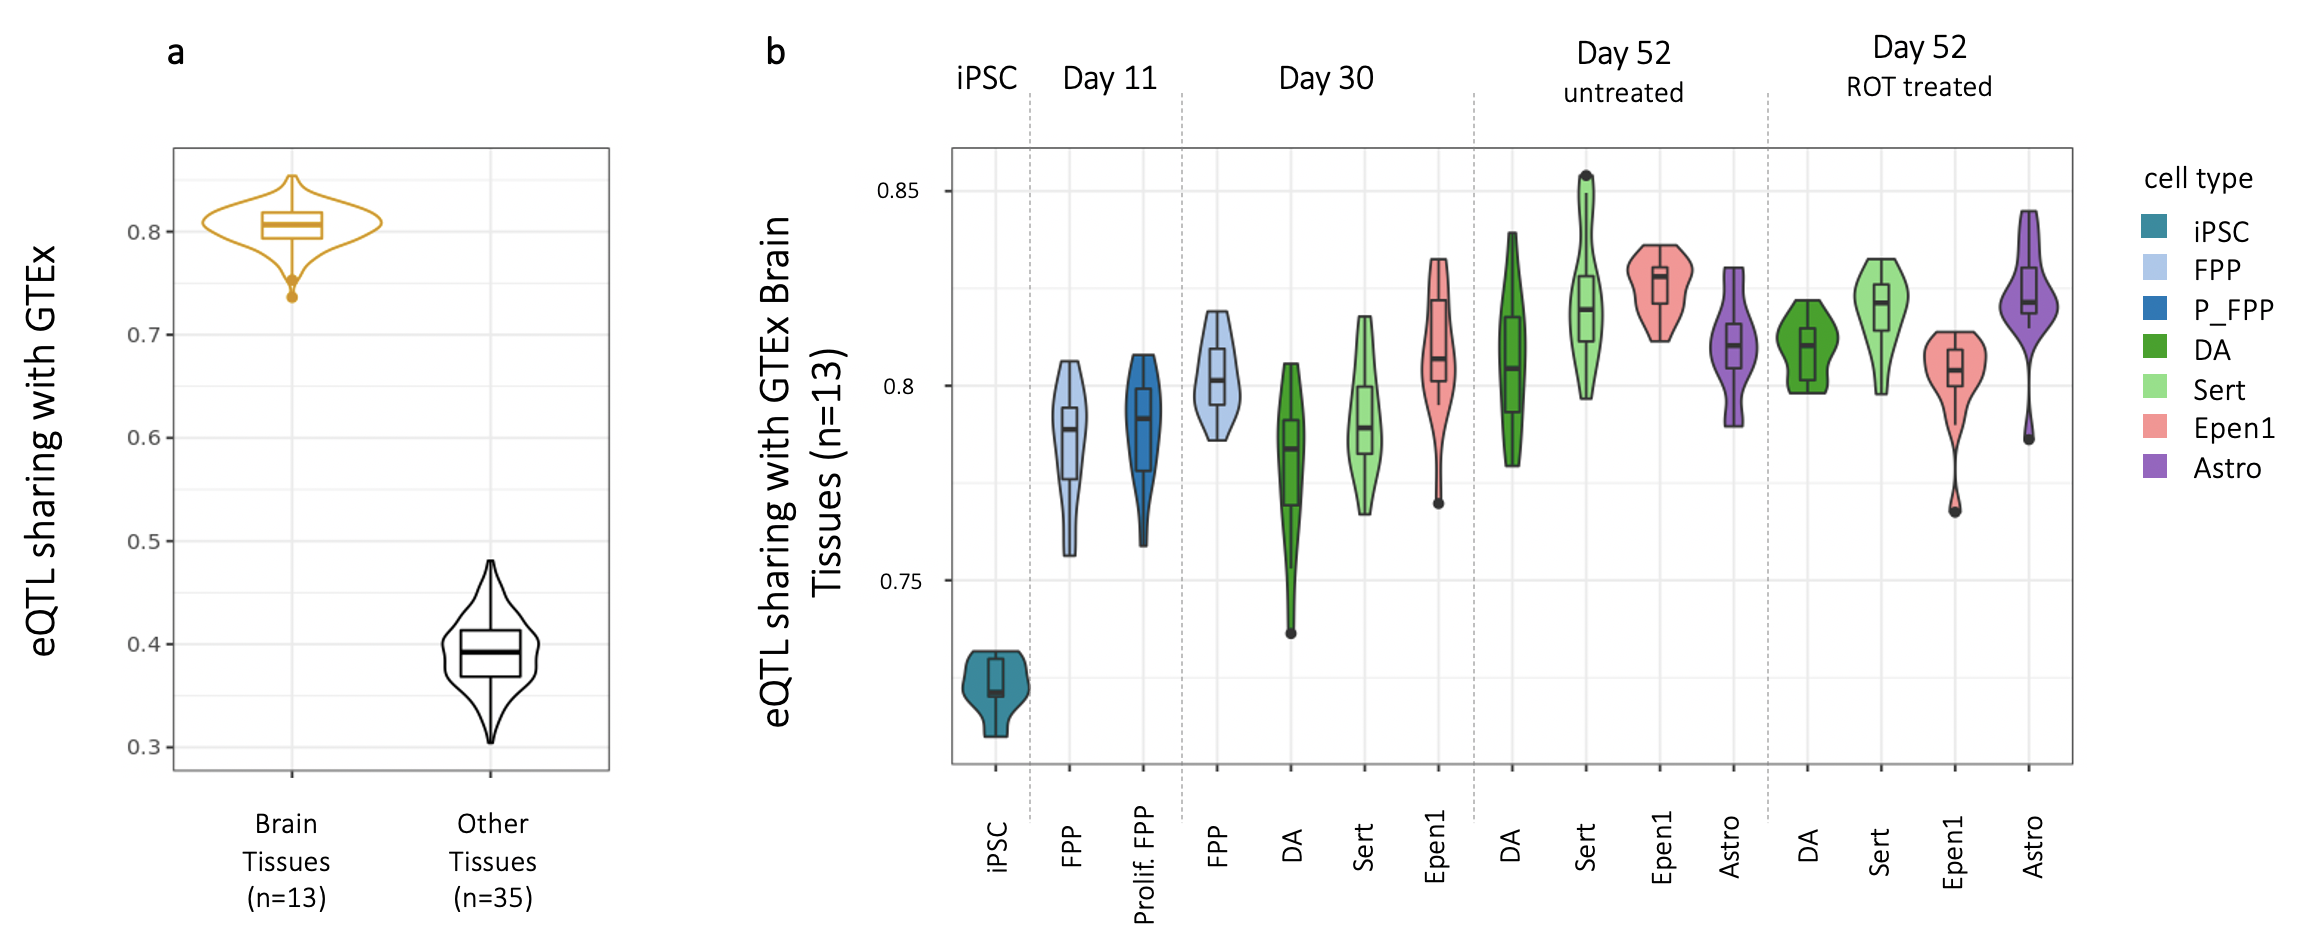
\includegraphics[width=16cm]{Chapter5/Fig/neuroseq_mashr.png}
\caption[GTEx sharing]{\textbf{Brain sharing is higher than non-brain sharing, and it increases over time}.\\
(a) Box plots indicating the amount of sharing as quantified by MASHR \cite{urbut2019flexible} of our 14 eQTL maps considered together, with each of the GTEx brain tissues (yellow, n=13) and with each of other (non-brain) GTEx tissues (black, n=35).
(b) Sharing of eQTL signals discovered in iPSCs and in our study (for each of our 14 cell types and conditions), with \textit{in vivo} brain eQTL maps (from GTEx). 
Violin plots show the extent of eQTL sharing with each of 13 GTEx brain eQTL maps.
Astro: Astrocyte-like, DA: Midbrain dopaminergic neurons, Epen1: Ependymal-like, FPP: Floor Plate Progenitors, iPSC: induced pluripotent stem cells, P\_FPP: Proliferating FPP, Sert: Serotonergic-like neurons.}
\label{fig:neuroseq_and_gtex_brain_sharing}
\end{figure}

This result provides confidence that eQTL discovered in iPSC-derived neuronal cell types mimic eQTL maps from \textit{in vivo} tissues. 
Consistent with the trend of increased sharing of eQTL signal, we also observed that the fraction of eQTL that are not represented in GTEx brain tissues decreases as the cells become increasingly mature. 
In particular, we identified 2,366 eQTL that could not be detected in GTEx brain tissues (q value > 0.05 in any of the 13 tissues), demonstrating the utility of iPSC and scRNA-seq analysis to assess previously unexplored cell populations and therein discover regulatory changes in disease associated genes. \\

Finally, we note that quantifying the amount of sharing of eQTL signal is a notoriously difficult problem.
As mentioned, MASHR considers only genes assessed in all conditions analysed. 
As a result, the degree of sharing may be inflated, because only relatively few highly expressed genes are included in the analysis, and those are more likely to be common eQTL. 
In particular using scRNA-seq we can assay fewer genes (as compared to bulk), thus the number of genes that we can assess in our single cell maps becomes the limiting factor in terms of genes included in the analysis (i.e. 8,706/8,738 genes assessed in all of our maps are also assessed in all GTEx brain maps).
On the other hand, as a complementary strategy to quantify eQTL sharing, we have also considered conventional definitions of eQTL replication, based on nominal significance of lead eQTL variants discovered in each of the 13 GTEx brain tissue eQTL maps, in each of our 14 eQTL maps (\textbf{Fig. \ref{fig:neuroseq_and_gtex_rediscovery}}).
Notably, this comparison allows for teasing apart lack of replication versus lack of assessment of an eGene because of difference in expression. We found that of the eGenes identified at FDR<5\% in each of the GTEx maps, approximately 50\% were tested in our different maps (\textbf{Fig. \ref{fig:neuroseq_and_gtex_rediscovery}}, panel a).
For the shared fraction of genes assessed, 20-40\% eQTL were nominally significant (p value < 0.05) across our 14 maps.
Cumulatively, this means that 10-20\% of the eQTL from a GTEx brain map could be re-discovered in our single cell maps (\textbf{Fig. \ref{fig:neuroseq_and_gtex_rediscovery}}, panel b).

\begin{figure}[h]
\centering
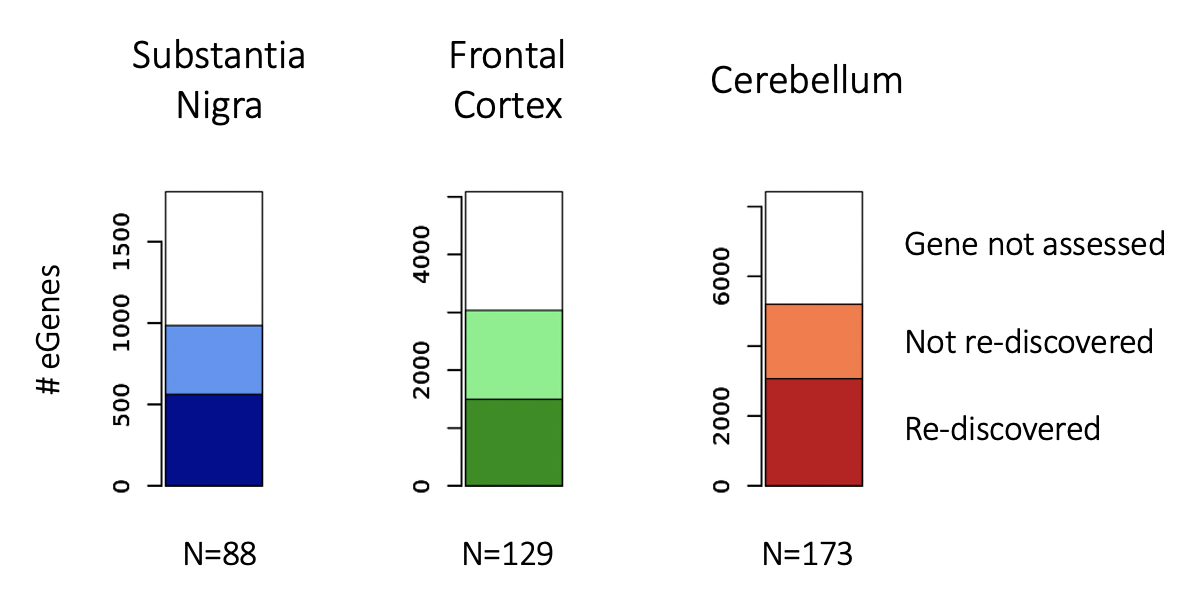
\includegraphics[width=13cm]{Chapter5/Fig/neuroseq_rediscovering_gtex_brain.png}
\caption[Rediscovery of GTEx brain eQTL maps]{\textbf{Rediscovery of GTEx brain eQTL maps}.\\
(a)Fraction of GTEx brain eGenes that could be assessed in each of the considered contexts (cell type-conditions). 
(b) Fraction of GTEx brain eQTL that were replicated in this study (nominal p value < 0.05; fraction relative to the set of assessed genes from a).
Astro: Astrocyte-like, DA: Midbrain dopaminergic neurons, Epen1: Ependymal-like, FPP: Floor Plate Progenitors, P\_FPP: Proliferating FPP, Sert: Serotonergic-like neurons.}
\label{fig:neuroseq_and_gtex_rediscovery}
\end{figure}

\clearpage

\section{Colocalisation of eQTL with disease risk variants}
\label{sec:neuroseq_coloc}

The identified cell-type specific eQTL maps across different differentiation contexts provide an exciting opportunity to improve our understanding of human disease traits and their genetic risk factors identified by GWA studies.
To systematically test for colocalisation events (\textbf{page \pageref{sec:eqtl_gwas}}), we applied COLOC \cite{giambartolomei2014bayesian} to the summary statistics from 25 neurological traits\footnote{including Parkinson's disease, Alzheimer's disease, schizophrenia, bipolar disorder, neuroticism, depression, and other behaviour and intelligence-related traits, see \textbf{Table \ref{tab:coloc_neuro_traits}}.}, eQTL discovered in our study, as well as eQTL obtained from GTEx (v7) \cite{gtex2017genetic}.\\

In total, we identified 1,284 eQTL in our study with evidence of colocalisation (PP4>0.5) with at least one disease trait, 597 of which were found only in our dataset. 
This corresponds to an additional >10\% of colocalisation events of GWAS variants compared to eQTL across all GTEx tissues (5,028 across 48 tissues, \textbf{Fig. \ref{fig:neuroseq_coloc_overview}}). 
Notably, 401 (67\%) of the colocalisations in our data were associated with eQTL detected in later differentiation stages (day 52) or upon stimulation (day 52 ROT).\\

\begin{figure}[h]
\centering
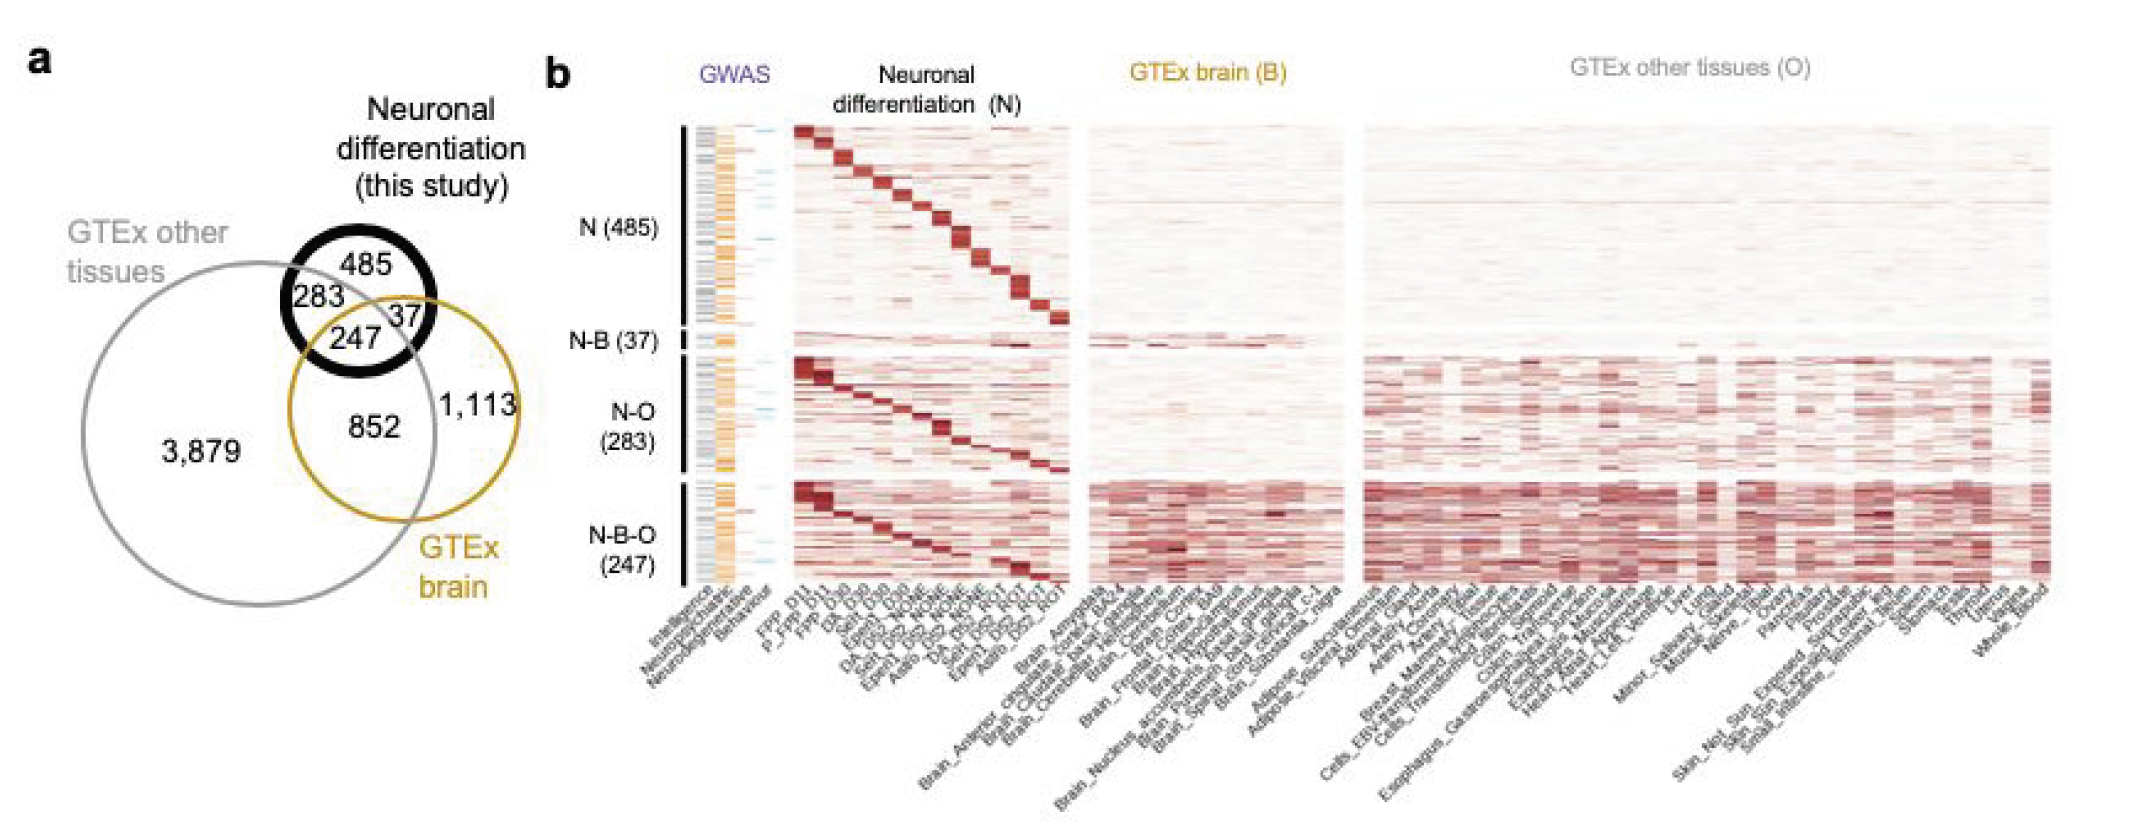
\includegraphics[width=16cm]{Chapter5/Fig/neuroseq_coloc_overview.png}
\caption[Coloc overview]{\textbf{Coloc overview}.\\
Figure by Natsuhiko Kumasaka.
Overview of colocalisation analysis between our eQTL maps and 25 neuro-related GWAS traits. 
(left) Venn diagram showing the numbers of colocalisation events overlapping between our study, GTEx brain and GTEx non brain tissues. 
(right) Heatmap showing the posterior probability of colocalisation (PP4 from COLOC \cite{giambartolomei2014bayesian}) for our eQTL that colocalised with one or more GWAS traits. 
N: Neuronal differentiation (this study), B: GTEx Brain tissues, O: Other GTEx tissues.}
\label{fig:neuroseq_coloc_overview}
\end{figure}

\newpage

Among the most interesting colocalisation events was an eQTL for \textit{SFXN5}, a mitochondrial amino-acid transporter, which was specific to the rotenone-stimulated serotonergic neurons at day 52, and which colocalised with a Schizophrenia hit (PP4 = 0.78, \textbf{Fig. \ref{fig:neuroseq_coloc_example1}}). 
Exposure to rotenone is known to induce oxidative stress by inhibiting the mitochondrial respiratory chain complex I \cite{palmer1968studies, betarbet2000chronic}. 
We therefore speculate that the specific genetic signal observed for the mitochondrial gene \textit{SFXN5} in serotonergic neurons is a possible factor modulating environmental stress response.

\begin{figure}[h]
\centering
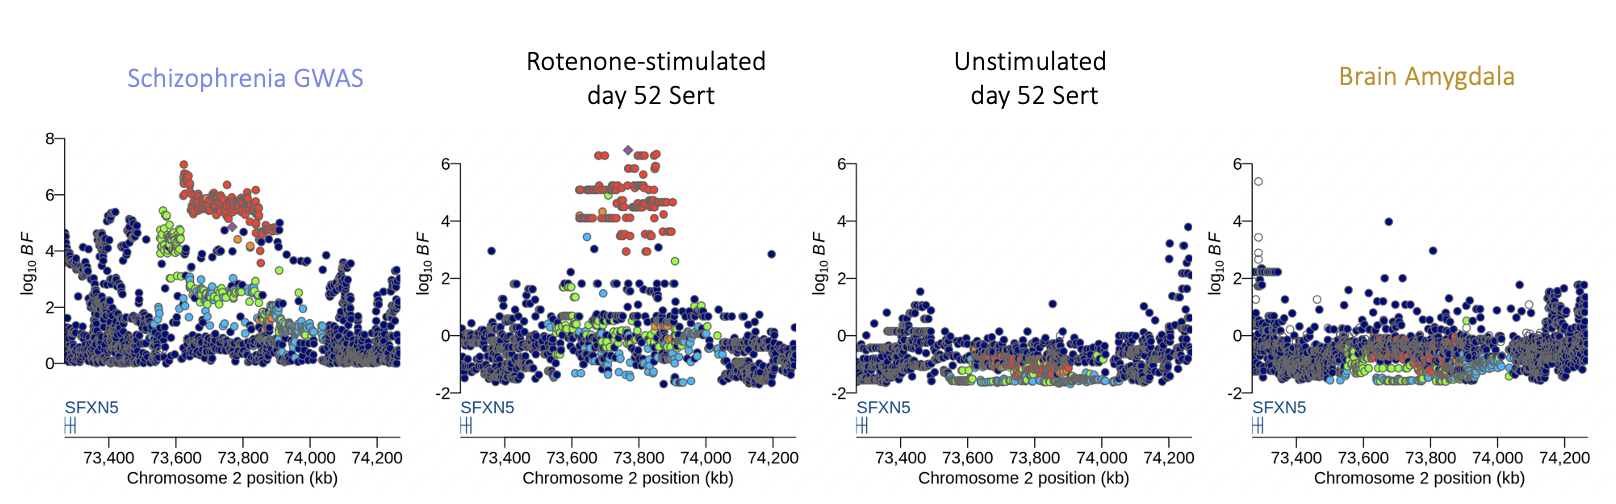
\includegraphics[width=15.5cm]{Chapter5/Fig/neuroseq_coloc_example1_SFXN5.png}
\caption[First example of colocalisation]{\textbf{A colocalisation event between a rotenone-specific eQTL and schizophrenia}.\\
Figure by Natsuhiko Kumasaka. Locus zoom plots around the \textit{SFXN5} gene. 
The Schizophrenia GWAS association (left) is colocalised with the eQTL in rotenone-stimulated serotonergic-like neurons at day 52 (second panel from the left). 
No colocalisation signal was found in unstimulated serotonergic-like neurons at day 52 (third panel from the left) or any other brain GTEx tissues as illustrated here with GTEx Brain Amygdala (rightmost panel). 
The lead variant is indicated with a purple diamond and other points were coloured according to the LD index ($r^2$ value) with the lead variant.}
\label{fig:neuroseq_coloc_example1}
\end{figure}

Another example that colocalised with a Schizophrenia GWAS variant was an eQTL for
\textit{FGFR1}, detected both in proliferating and non proliferating floor plate progenitors at day 11 (PP4 = 0.93 and 0.88 respectively, \textbf{Fig \ref{fig:neuroseq_coloc_example2}}) . 
Previous studies have shown that nuclear \textit{FGFR1} plays a key role in regulating neural stem cell proliferation and central nervous system development, in part, by binding to the promoters of genes that control the transition from proliferation to cell differentiation \cite{ma2009molecular}. 
Additionally, it was shown that altered \textit{FGFR1} signaling was linked to the progression of the cortical malformation observed in schizophrenia \cite{stachowiak2017cerebral}.\\

\begin{figure}[h]
\centering
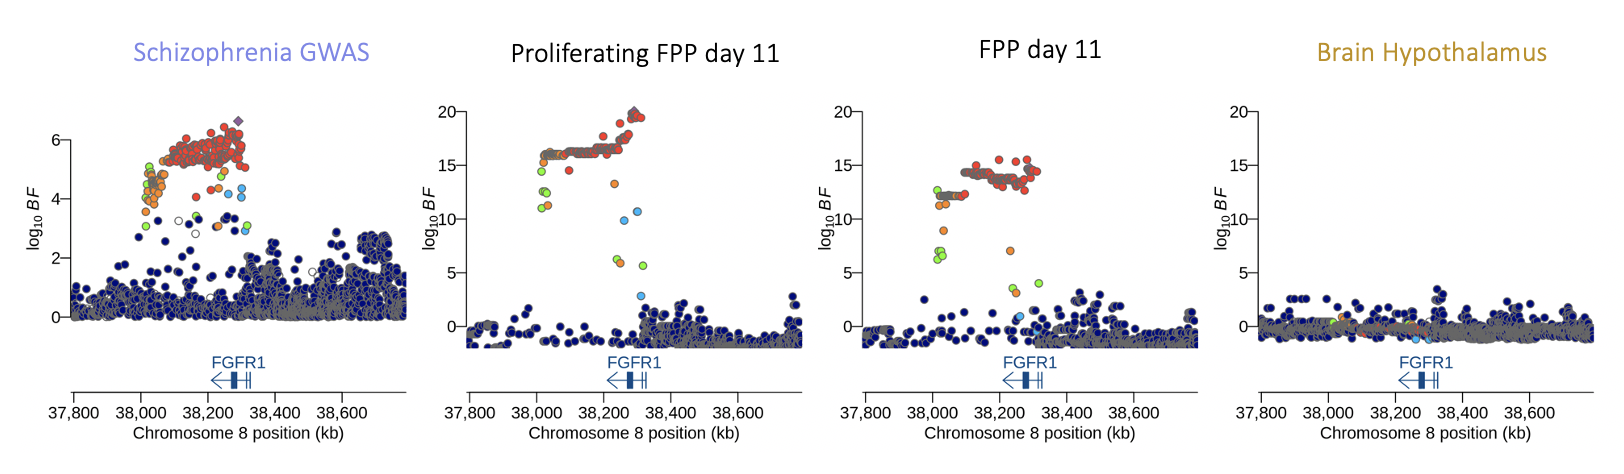
\includegraphics[width=15.5cm]{Chapter5/Fig/neuroseq_coloc_example2_FGFR1.png}
\caption[Second example of colocalisation]{\textbf{A schizophrenia colocalisation event with a developmental eQTL}.\\
Figure by Natsuhiko Kumasaka. A midbrain progenitor-specific eQTL for \textit{FGFR1} associated with schizophrenia. 
We identified a colocalisation event with this eQTL in both proliferating (second panel from the left) and non-proliferating floor plate progenitors (third panel from the left) at day 11. 
No colocalisation was found in any other cell type from our study (not shown) nor in any brain GTEx tissues (shown with GTEx Brain Hypothalamus, rightmost panel).}
\label{fig:neuroseq_coloc_example2}
\end{figure}

\newpage

These examples suggest that a combination of genetic and environmental factors during early development might contribute to schizophrenia pathology and illustrate how these data represent a valuable resource to understand the molecular basis of complex neurological diseases.

\section{Discussion}
\label{sec:neuroseq_discussion}

The characterisation of the function of human trait-associated genetic variation requires large-scale studies, performed in disease-relevant cell types and states. 
Here, we demonstrate how human iPSCs can be efficiently profiled at scale throughout a 52 day-long differentiation to a midbrain neuronal cell fate. \\

First, we demonstrate high heterogeneity of cell types generated by this protocol (\textbf{Fig. \ref{fig:neuroseq_overview}}), and uncover a highly reproducible (\textbf{Fig. \ref{fig:neuroseq_diff_eff_replication}, \ref{fig:neuroseq_organoids}}), cell line-intrinsic neuronal differentiation bias (\textbf{Fig. \ref{fig:neuroseq_diff_efficiency}}).
Next, we show how this bias can be robustly predicted using gene expression profiling at iPSC state (\textbf{Fig. \ref{fig:neuroseq_ips_expression_signature}}). 
This is an important step towards the optimised design of future large-scale iPSC experiments, where cell lines can be rationally selected a priori without the need for laborious testing of differentiation capacity. \\

Indeed, the `quality' of human iPS cells has been carefully examined by several studies using both genetic and functional genomic data \cite{muller2011bioinformatic, international2018assessment, tsankov2015qpcr, bock2011reference}, see also \textbf{section \ref{sec:ipsc_characterise}}. 
Despite these efforts, variation in differentiation potential between cell lines has been widely acknowledged, yet poorly understood. 
To the best of our knowledge, the work we presented here is the first effort to systematically survey differentiation biases at the scale of an entire iPSC bank. 
To address this question, we leveraged the detailed phenotyping of cell lines in the HipSci bank.
We excluded the cell type of origin hypothesis \cite{hu2016effects} in this instance since all HipSci lines were derived from fibroblasts.
Moreover, we observed rather weak associations between neuronal differentiation efficiency and other biological factors, including sex and X chromosome activation status, which has been described as relevant for other differentiation lineages (i.e. endoderm lineage, see \textbf{Chapter \ref{chapter4}} and \cite{cuomo2020single}).
In this work, we focused on the cell-line effects, that were especially prevalent (\textbf{Fig. \ref{fig:neuroseq_diff_eff_vca}}), but further investigation into the effects of sex and X chromosome inactivation (as well donor ethnicity, although that could not have been assessed in this study) is left for future work. \\

Our analysis indicates that the reduced production of neurons was best correlated with increased abundance of a specific subpopulation (cluster 2) of iPS cells that express the transcription factor \textit{UTF1} and other genes at elevated levels (\textbf{Fig. \ref{fig:neuroseq_ips_sc_genes}}).
Counter-intuitively, the proportion of cells in this subpopulation was positively correlated with the proportion of neuroblast cells on day 11, but lower fractions of dopaminergic and serotonergic-like neurons at later stages of differentiation. 
One possible explanation is that cell lines that commit earlier to a neuronal fate disproportionately lose neurons upon passaging at day 20 (\textbf{Fig. \ref{fig:neuroseq_experimental_design}}, cells are passaged at day 20 as from original protocol \cite{kriks2011dopamine}; this would explain the lack of clear differences between lines at day 11, with instead divergence appearing at the day 30 time point and then becoming even more evident by day 52). \\

In alternative, cluster 2 may preferentially differentiate to radial glial cells which are more prone to switch to an astroglial and ependymal differentiation programme \cite{spassky2005adult}. 
In support of this hypothesis, we identified several genes that were upregulated in cluster 2, including \textit{SIX3}, \textit{MT1F} and \textit{PITX2}, that are thought to play a role in astrocyte and ependymal cell biogenesis \cite{lavado2011six3, michael2011up, jacquet2009foxj1}. \\

A second implication of our study is that, despite growth competition between cell lines, pooled experiments retain sufficient cells per donor to carry out genetic analysis, even following extended periods in culture. 
Although cells from different lines were pooled in similar numbers, we observed extensive variation throughout our differentiation experiments in the numbers of cells produced by different lines. 
For example, 50\% of the cells we sequenced were produced by only 12\% of lines.
As we have demonstrated, this was an important effect to take into account in our eQTL analysis (\textbf{Fig. \ref{fig:neuroseq_eqtl_improved_power}}).
Future technical improvements, for instance more precise matching of growth rates of cell lines within pools, or line selection based on predicted differentiation efficiency using markers in the iPSC state may further increase the utility of multiplexed iPSC differentiation experiments.\\

Finally, we could map eQTL across several neuronal cell types and in response to oxidative stress (\textbf{Fig. \ref{fig:neuroseq_eqtl}}).
As we have seen, in order to understand the functional role of trait-associated variants it is crucial to perform genetic analyses in relevant cell types.
Indeed, as a community, we have largely been unable to identify genetic variants that drive expression changes in narrowly-defined cell populations.
This is due to our reliance on tissue-level data (e.g. GTEx), our incomplete knowledge of cell populations present in a tissue, or because rare cell populations do not provide enough substrate for common genomics assays. \\

Our analysis attempts to be a step towards investigating cell type-specific genetic effect, which are often masked in tissue-level assays.
Indeed, despite a modest sample size, our study reveals a disproportionately large number of novel colocalisations between neurological traits and diseases and eQTL (\textbf{Fig. \ref{fig:neuroseq_coloc_overview}}) compared with GTEx tissues of equivalent sample size. 
For example, the number of novel trait/disease-eQTL colocalisations added by GTEx liver or cerebellar hemisphere (n=208, 215 respectively) are 80 and 107, respectively, compared to 597 in this study. 
A simple explanation for this result is that our experiment profiled expression states that are hard to capture using post-mortem tissue, including time points during neuronal differentiation and rotenone exposure. \\

Additionally, the single-cell resolution of our study enabled the detection of many eQTL that were specific to individual cell types, or could only be detected upon stimulation (\textbf{Fig. \ref{fig:neuroseq_eqtl_examples}}).
These signals, while present, are challenging to detect in bulk tissue because the relevant cell types are often rare. 
Combined, these results suggest that many `missing', disease-relevant eQTL remain to be discovered using single cell profiling of both primary tissues and \textit{in vitro} models.